

%\documentclass[conference,a4paper]{IEEEtran}
\documentclass[journal]{IEEEtran}

\usepackage[pdftex]{graphicx}

\usepackage{amsmath}

% \interdisplaylinepenalty=2500
% \ifCLASSOPTIONcompsoc
%   \usepackage[caption=false,font=normalsize,labelfont=sf,textfont=sf]{subfig}
% \else
%   \usepackage[caption=false,font=footnotesize]{subfig}
% \fi

%=======================================================
\usepackage{currfile}
\usepackage{standalone}
\usepackage{tikz}
\usepackage{tikzscale}
\usetikzlibrary{decorations.markings}
\usepackage{pgfplots}
\pgfplotsset{compat=newest,grid=major,major grid style={black,dotted},every
	axis plot/.append style={thick}}
%===================================================
% correct bad hyphenation here
\hyphenation{op-tical net-works semi-conduc-tor}
\hyphenation{re-so-na-tors}

% bibliography management
%\usepackage[style = ieee]{biblatex}
%\addbibresource{literature.bib}

% units
\usepackage{siunitx}
\DeclareSIUnit{\belisotropic}{Bi}
\DeclareSIUnit{\dBi}{\deci\belisotropic}
\DeclareSIUnit{\bit}{bit}

% tables
\usepackage{booktabs}
%\usepackage{caption}
%\usepackage[table,xcdraw]{xcolor}

 \usepackage{flushend}
\usepackage{lipsum}

% Acronyms
\usepackage[acronym]{glossaries}
%\usepackage{subcaption}

\begin{acronym}[LTE-Advanced]%\addtolength{\itemsep}{-0.5\baselineskip}
\acro{GB2D}{gridless blind deconvolution and demixing}
  \acro{ISAC}{integrated (radar) sensing and communications}
  \acro{2G}{Second Generation}
  \acro{6G}{Sixth Generation}
  \acro{3-DAP}{3-Dimensional Assignment Problem}
  \acro{AA}{Antenna Array}
  \acro{AC}{Admission Control}
  \acro{AD}{Attack-Decay}
  \acro{ADC}{analog-to-digital conversion}
  \acro{ADMM}{alternating direction method of multipliers}
  \acro{ADSL}{Asymmetric Digital Subscriber Line}
  \acro{AHW}{Alternate Hop-and-Wait}
  \acro{AI}{Artificial Intelligence}
  \acro{AirComp}{Over-the-air computation}
  \acro{AMC}{Adaptive Modulation and Coding}
  \acro{AP}{\LU{A}{a}ccess \LU{P}{p}oint}
  \acro{APA}{Adaptive Power Allocation}
  \acro{ARMA}{Autoregressive Moving Average}
  \acro{ARQ}{\LU{A}{a}utomatic \LU{R}{r}epeat \LU{R}{r}equest}
  \acro{ATES}{Adaptive Throughput-based Efficiency-Satisfaction Trade-Off}
  \acro{AWGN}{additive white Gaussian noise}
  \acro{BAA}{\LU{B}{b}roadband \LU{A}{a}nalog \LU{A}{a}ggregation}
  \acro{BB}{Branch and Bound}
  \acro{BCD}{block coordinate descent}
  \acro{BD}{Block Diagonalization}
  \acro{BER}{Bit Error Rate}
  \acro{BF}{Best Fit}
  \acro{BFD}{bidirectional full duplex}
  \acro{BLER}{BLock Error Rate}
  \acro{BPC}{Binary Power Control}
  \acro{BPSK}{Binary Phase-Shift Keying}
  \acro{BRA}{Balanced Random Allocation}
  \acro{BS}{base station}
  \acro{BSUM}{block successive upper-bound minimization}
  \acro{CAP}{Combinatorial Allocation Problem}
  \acro{CAPEX}{Capital Expenditure}
  \acro{CBF}{Coordinated Beamforming}
  \acro{CBR}{Constant Bit Rate}
  \acro{CBS}{Class Based Scheduling}
  \acro{CC}{Congestion Control}
  \acro{CDF}{Cumulative Distribution Function}
  \acro{CDMA}{Code-Division Multiple Access}
  \acro{CE}{\LU{C}{c}hannel \LU{E}{e}stimation}
  \acro{CL}{Closed Loop}
  \acro{CLPC}{Closed Loop Power Control}
  \acro{CML}{centralized machine learning}
  \acro{CNR}{Channel-to-Noise Ratio}
  \acro{CNN}{\LU{C}{c}onvolutional \LU{N}{n}eural \LU{N}{n}etwork}
  \acro{CPA}{Cellular Protection Algorithm}
  \acro{CPICH}{Common Pilot Channel}
  \acro{CoCoA}{\LU{C}{c}ommunication efficient distributed dual \LU{C}{c}oordinate \LU{A}{a}scent}
  \acro{CoMAC}{\LU{C}{c}omputation over \LU{M}{m}ultiple-\LU{A}{a}ccess \LU{C}{c}hannels}
  \acro{CoMP}{Coordinated Multi-Point}
  \acro{CQI}{Channel Quality Indicator}
  \acro{CRM}{Constrained Rate Maximization}
	\acro{CRN}{Cognitive Radio Network}
  \acro{CS}{Coordinated Scheduling}
  \acro{CSI}{\LU{C}{c}hannel \LU{S}{s}tate \LU{I}{i}nformation}
  \acro{CSMA}{\LU{C}{c}arrier \LU{S}{s}ense \LU{M}{m}ultiple \LU{A}{a}ccess}
  \acro{CUE}{Cellular User Equipment}
  \acro{D2D}{device-to-device}
  \acro{DAC}{digital-to-analog converter}
  \acro{DC}{direct current}
  \acro{DCA}{Dynamic Channel Allocation}
  \acro{DE}{Differential Evolution}
  \acro{DFT}{Discrete Fourier Transform}
%  \acro{DIST}{Distance-based Grouping}
  \acro{DIST}{Distance}
  \acro{DL}{downlink}
  \acro{DMA}{Double Moving Average}
  \acro{DML}{Distributed Machine Learning}
  \acro{DMRS}{demodulation reference signal}
  \acro{D2DM}{D2D Mode}
  \acro{DMS}{D2D Mode Selection}
  \acro{DNN}{Deep Neural Network}
  \acro{DPC}{Dirty Paper Coding}
  \acro{DRA}{Dynamic Resource Assignment}
  \acro{DSA}{Dynamic Spectrum Access}
  \acro{DSGD}{\LU{D}{d}istributed \LU{S}{s}tochastic \LU{G}{g}radient \LU{D}{d}escent}
  \acro{DSM}{Delay-based Satisfaction Maximization}
  \acro{ECC}{Electronic Communications Committee}
  \acro{EFLC}{Error Feedback Based Load Control}
  \acro{EI}{Efficiency Indicator}
  \acro{eNB}{Evolved Node B}
  \acro{EPA}{Equal Power Allocation}
  \acro{EPC}{Evolved Packet Core}
  \acro{EPS}{Evolved Packet System}
  \acro{E-UTRAN}{Evolved Universal Terrestrial Radio Access Network}
  \acro{ES}{Exhaustive Search}
  %\acro{FD}{full duplex}
  \acro{FC}{\LU{F}{f}usion \LU{C}{c}enter}
  \acro{FD}{\LU{F}{f}ederated \LU{D}{d}istillation}
  \acro{FDD}{frequency division duplex}
  \acro{FDM}{Frequency Division Multiplexing}
  \acro{FDMA}{\LU{F}{f}requency \LU{D}{d}ivision \LU{M}{m}ultiple \LU{A}{a}ccess}
  \acro{FedAvg}{\LU{F}{f}ederated \LU{A}{a}veraging}
  \acro{FER}{Frame Erasure Rate}
  \acro{FF}{Fast Fading}
  \acro{FL}{Federated Learning}
  \acro{FSB}{Fixed Switched Beamforming}
  \acro{FST}{Fixed SNR Target}
  \acro{FTP}{File Transfer Protocol}
  \acro{GA}{Genetic Algorithm}
  \acro{GBR}{Guaranteed Bit Rate}
  \acro{GD}{gradient descent}
  \acro{GLR}{Gain to Leakage Ratio}
  \acro{GOS}{Generated Orthogonal Sequence}
  \acro{GPL}{GNU General Public License}
  \acro{GRP}{Grouping}
  \acro{HARQ}{Hybrid Automatic Repeat Request}
  \acro{HD}{half-duplex}
  \acro{HMS}{Harmonic Mode Selection}
  \acro{HOL}{Head Of Line}
  \acro{HSDPA}{High-Speed Downlink Packet Access}
  \acro{HSPA}{High Speed Packet Access}
  \acro{HTTP}{HyperText Transfer Protocol}
  \acro{ICMP}{Internet Control Message Protocol}
  \acro{ICI}{Intercell Interference}
  \acro{ID}{Identification}
  \acro{IETF}{Internet Engineering Task Force}
  \acro{ILP}{Integer Linear Program}
  \acro{JRAPAP}{Joint RB Assignment and Power Allocation Problem}
  \acro{UID}{Unique Identification}
  \acro{IID}{\LU{I}{i}ndependent and \LU{I}{i}dentically \LU{D}{d}istributed}
  \acro{IIR}{Infinite Impulse Response}
  \acro{ILP}{Integer Linear Problem}
  \acro{IMT}{International Mobile Telecommunications}
  \acro{INV}{Inverted Norm-based Grouping}
  \acro{IoT}{Internet of Things}
%  \acro{IP}{Internet Protocol}
  \acro{IP}{Integer Programming}
  \acro{IPv6}{Internet Protocol Version 6}
  \acro{IQ}{in-phase quadrature}
  \acro{ISD}{Inter-Site Distance}
  \acro{ISI}{Inter Symbol Interference}
  \acro{ITU}{International Telecommunication Union}
  \acro{JAFM}{joint assignment and fairness maximization}
  \acro{JAFMA}{joint assignment and fairness maximization algorithm}
  \acro{JOAS}{Joint Opportunistic Assignment and Scheduling}
  \acro{JOS}{Joint Opportunistic Scheduling}
  \acro{JP}{Joint Processing}
	\acro{JS}{Jump-Stay}
  \acro{KKT}{Karush-Kuhn-Tucker}
  \acro{L3}{Layer-3}
  \acro{LAC}{Link Admission Control}
  \acro{LA}{Link Adaptation}
  \acro{LC}{Load Control}
  \acro{LDC}{\LU{L}{l}earning-\LU{D}{d}riven \LU{C}{c}ommunication}
  \acro{LOS}{line of sight}
  \acro{LP}{Linear Programming}
  \acro{LTE}{Long Term Evolution}
	\acro{LTE-A}{\ac{LTE}-Advanced}
  \acro{LTE-Advanced}{Long Term Evolution Advanced}
  \acro{M2M}{Machine-to-Machine}
  \acro{MAC}{multiple access channel}
  \acro{MANET}{Mobile Ad hoc Network}
  \acro{MC}{Modular Clock}
  \acro{MCS}{Modulation and Coding Scheme}
  \acro{MDB}{Measured Delay Based}
  \acro{MDI}{Minimum D2D Interference}
  \acro{MF}{Matched Filter}
  \acro{MG}{Maximum Gain}
  \acro{MH}{Multi-Hop}
  \acro{MIMO}{\LU{M}{m}ultiple \LU{I}{i}nput \LU{M}{m}ultiple \LU{O}{o}utput}
  \acro{MINLP}{mixed integer nonlinear programming}
  \acro{MIP}{Mixed Integer Programming}
  \acro{MISO}{multiple input single output}
  \acro{ML}{Machine Learning}
  \acro{MLWDF}{Modified Largest Weighted Delay First}
  \acro{MME}{Mobility Management Entity}
  \acro{MMSE}{minimum mean squared error}
  \acro{MOS}{Mean Opinion Score}
  \acro{MPF}{Multicarrier Proportional Fair}
  \acro{MRA}{Maximum Rate Allocation}
  \acro{MR}{Maximum Rate}
  \acro{MRC}{Maximum Ratio Combining}
  \acro{MRT}{Maximum Ratio Transmission}
  \acro{MRUS}{Maximum Rate with User Satisfaction}
  \acro{MS}{Mode Selection}
  \acro{MSE}{\LU{M}{m}ean \LU{S}{s}quared \LU{E}{e}rror}
  \acro{MSI}{Multi-Stream Interference}
  \acro{MTC}{Machine-Type Communication}
  \acro{MTSI}{Multimedia Telephony Services over IMS}
  \acro{MTSM}{Modified Throughput-based Satisfaction Maximization}
  \acro{MU-MIMO}{Multi-User Multiple Input Multiple Output}
  \acro{MU}{Multi-User}
  \acro{NAS}{Non-Access Stratum}
  \acro{NB}{Node B}
	\acro{NCL}{Neighbor Cell List}
  \acro{NLP}{Nonlinear Programming}
  \acro{NLOS}{non-line of sight}
  \acro{NMSE}{Normalized Mean Square Error}
  \acro{NN}{Neural Network}
  \acro{NOMA}{\LU{N}{n}on-\LU{O}{o}rthogonal \LU{M}{m}ultiple \LU{A}{a}ccess}
  \acro{NORM}{Normalized Projection-based Grouping}
  \acro{NP}{non-polynomial time}
  \acro{NRT}{Non-Real Time}
  \acro{NSPS}{National Security and Public Safety Services}
  \acro{O2I}{Outdoor to Indoor}
  \acro{OAC}{Over-the-Air Computation}
  \acro{OFDMA}{\LU{O}{o}rthogonal \LU{F}{f}requency \LU{D}{d}ivision \LU{M}{m}ultiple \LU{A}{a}ccess}
  \acro{OFDM}{Orthogonal Frequency Division Multiplexing}
  \acro{OFPC}{Open Loop with Fractional Path Loss Compensation}
	\acro{O2I}{Outdoor-to-Indoor}
  \acro{OL}{Open Loop}
  \acro{OLPC}{Open-Loop Power Control}
  \acro{OL-PC}{Open-Loop Power Control}
  \acro{OPEX}{Operational Expenditure}
  \acro{ORB}{Orthogonal Random Beamforming}
  \acro{JO-PF}{Joint Opportunistic Proportional Fair}
  \acro{OSI}{Open Systems Interconnection}
  \acro{PAIR}{D2D Pair Gain-based Grouping}
  \acro{PAPR}{Peak-to-Average Power Ratio}
  \acro{P2P}{Peer-to-Peer}
  \acro{PC}{Power Control}
  \acro{PCI}{Physical Cell ID}
  \acro{PDCCH}{physical downlink control channel}
  \acro{PDD}{penalty dual decomposition}
  \acro{PDF}{Probability Density Function}
  \acro{PER}{Packet Error Rate}
  \acro{PF}{Proportional Fair}
  \acro{P-GW}{Packet Data Network Gateway}
  \acro{PL}{Pathloss}
  \acro{PLL}{phase-locked Loop}
  \acro{PRB}{Physical Resource Block}
  \acro{PROJ}{Projection-based Grouping}
  \acro{ProSe}{Proximity Services}
%  \acro{PS}{Packet Scheduling}
%  \acro{PS}{phase shifter}
  \acro{PS}{\LU{P}{p}arameter \LU{S}{s}erver}
  \acro{PSO}{Particle Swarm Optimization}
  \acro{PUCCH}{physical uplink control channel}
  \acro{PZF}{Projected Zero-Forcing}
  \acro{QAM}{Quadrature Amplitude Modulation}
  \acro{QoS}{quality of service}
  \acro{QPSK}{Quadri-Phase Shift Keying}
  \acro{RAISES}{Reallocation-based Assignment for Improved Spectral Efficiency and Satisfaction}
  \acro{RAN}{Radio Access Network}
  \acro{RA}{Resource Allocation}
  \acro{RAT}{Radio Access Technology}
  \acro{RATE}{Rate-based}
  \acro{RB}{resource block}
  \acro{RBG}{Resource Block Group}
  \acro{REF}{Reference Grouping}
  \acro{RF}{radio frequency}
  \acro{RLC}{Radio Link Control}
  \acro{RM}{Rate Maximization}
  \acro{RNC}{Radio Network Controller}
  \acro{RND}{Random Grouping}
  \acro{RRA}{Radio Resource Allocation}
  \acro{RRM}{\LU{R}{r}adio \LU{R}{r}esource \LU{M}{m}anagement}
  \acro{RSCP}{Received Signal Code Power}
  \acro{RSRP}{reference signal receive power}
  \acro{RSRQ}{Reference Signal Receive Quality}
  \acro{RR}{Round Robin}
  \acro{RRC}{Radio Resource Control}
  \acro{RSSI}{received signal strength indicator}
  \acro{RT}{Real Time}
  \acro{RU}{Resource Unit}
  \acro{RUNE}{RUdimentary Network Emulator}
  \acro{RV}{Random Variable}
  \acro{SAC}{Session Admission Control}
  \acro{SCM}{Spatial Channel Model}
  \acro{SC-FDMA}{Single Carrier - Frequency Division Multiple Access}
  \acro{SD}{Soft Dropping}
  \acro{S-D}{Source-Destination}
  \acro{SDPC}{Soft Dropping Power Control}
  \acro{SDMA}{Space-Division Multiple Access}
  \acro{SDR}{semidefinite relaxation}
  \acro{SDP}{semidefinite programming}
  \acro{SER}{Symbol Error Rate}
  \acro{SES}{Simple Exponential Smoothing}
  \acro{S-GW}{Serving Gateway}
  \acro{SGD}{\LU{S}{s}tochastic \LU{G}{g}radient \LU{D}{d}escent}  
  \acro{SINR}{signal-to-interference-plus-noise ratio}
%   \acro{SI}{Satisfaction Indicator}
  \acro{SI}{self-interference}
  \acro{SIP}{Session Initiation Protocol}
  \acro{SISO}{\LU{S}{s}ingle \LU{I}{i}nput \LU{S}{s}ingle \LU{O}{o}utput}
  \acro{SIMO}{Single Input Multiple Output}
  \acro{SIR}{Signal to Interference Ratio}
  \acro{SLNR}{Signal-to-Leakage-plus-Noise Ratio}
  \acro{SMA}{Simple Moving Average}
  \acro{SNR}{\LU{S}{s}ignal-to-\LU{N}{n}oise \LU{R}{r}atio}
  \acro{SORA}{Satisfaction Oriented Resource Allocation}
  \acro{SORA-NRT}{Satisfaction-Oriented Resource Allocation for Non-Real Time Services}
  \acro{SORA-RT}{Satisfaction-Oriented Resource Allocation for Real Time Services}
  \acro{SPF}{Single-Carrier Proportional Fair}
  \acro{SRA}{Sequential Removal Algorithm}
  \acro{SRS}{sounding reference signal}
  \acro{SU-MIMO}{Single-User Multiple Input Multiple Output}
  \acro{SU}{Single-User}
  \acro{SVD}{Singular Value Decomposition}
  \acro{SVM}{\LU{S}{s}upport \LU{V}{v}ector \LU{M}{m}achine}
  \acro{TCP}{Transmission Control Protocol}
  \acro{TDD}{time division duplex}
  \acro{TDMA}{\LU{T}{t}ime \LU{D}{d}ivision \LU{M}{m}ultiple \LU{A}{a}ccess}
  \acro{TNFD}{three node full duplex}
  \acro{TETRA}{Terrestrial Trunked Radio}
  \acro{TP}{Transmit Power}
  \acro{TPC}{Transmit Power Control}
  \acro{TTI}{transmission time interval}
  \acro{TTR}{Time-To-Rendezvous}
  \acro{TSM}{Throughput-based Satisfaction Maximization}
  \acro{TU}{Typical Urban}
  \acro{UE}{\LU{U}{u}ser \LU{E}{e}quipment}
  \acro{UEPS}{Urgency and Efficiency-based Packet Scheduling}
  \acro{UL}{uplink}
  \acro{UMTS}{Universal Mobile Telecommunications System}
  \acro{URI}{Uniform Resource Identifier}
  \acro{URM}{Unconstrained Rate Maximization}
  \acro{VR}{Virtual Resource}
  \acro{VoIP}{Voice over IP}
  \acro{WAN}{Wireless Access Network}
  \acro{WCDMA}{Wideband Code Division Multiple Access}
  \acro{WF}{Water-filling}
  \acro{WiMAX}{Worldwide Interoperability for Microwave Access}
  \acro{WINNER}{Wireless World Initiative New Radio}
  \acro{WLAN}{Wireless Local Area Network}
  \acro{WMMSE}{weighted minimum mean square error}
  \acro{WMPF}{Weighted Multicarrier Proportional Fair}
  \acro{WPF}{Weighted Proportional Fair}
  \acro{WSN}{Wireless Sensor Network}
  \acro{WWW}{World Wide Web}
  \acro{XIXO}{(Single or Multiple) Input (Single or Multiple) Output}
  \acro{ZF}{Zero-Forcing}
  \acro{ZMCSCG}{Zero Mean Circularly Symmetric Complex Gaussian}
\end{acronym}
%\end{singlespace}



% lists
\usepackage{enumerate}

%%%%Added by Arash %%%%
\usepackage{xcolor}
\newcommand{ \red} [ 1]{{\color{red}#1}}
\newcommand{ \blue} [ 1]{{\color{blue}#1}}

\newcommand{\ara}[1]{{\color{red}AA: #1}}
\newcommand{\vahid}[1]{{\color{DarkGreen}VJ: #1}}
\definecolor{DarkGreen}{RGB}{0,150,0}
\newcommand{\alejandro}[1]{{\color{Orange}AJS: #1}}
\definecolor{Orange}{RGB}{245,100,10}

\usepackage[normalem]{ulem}

%% Added by Alejandro
\usepackage{todonotes}

\begin{document}

\title{Reconfigurable Intelligent Surfaces with Liquid Crystal Technology: A Hardware Design and Communication Perspective}

\author{Alejandro Jim\'enez-S\'aez,  Arash Asadi,  Robin Neuder, Mohamadreza Delbari, and Vahid Jamali
%
\thanks{A. Jim\'enez-S\'aez and R. Neuder  are with the Institute of Microwave Engineering and Photonics at Technical University of Darmstadt, Darmstadt, Germany (e-mail:  \{alejandro.jimenez\_saez, robin.neuder\}@tu-darmstadt.de).} 
%
\thanks{A. Asadi is with the Wireless Communication and Sensing Lab at Technical University of Darmstadt, Darmstadt, Germany (e-mail:  aasadi@wise.tu-darmstadt.de).} 
%
\thanks{M. Delbari and V. Jamali are with the Resilient Communication Systems Lab at Technical University of Darmstadt, Darmstadt, Germany (e-mail:  \{mohamadreza.delbari, vahid.jamali\}@tu-darmstadt.de).} 
%
}


% \author{Alejandro Jim\'enez-S\'aez\IEEEauthorrefmark{1},
%         Arash Asadi\IEEEauthorrefmark{2},
%         Robin Neuder\IEEEauthorrefmark{1}, 
%         Mohamadreza Delbari\IEEEauthorrefmark{3}, and
%         Vahid Jamali\IEEEauthorrefmark{3}% <-this % stops a space
%         %Dongwei Wang\IEEEauthorrefmark{1},
%         %and Rolf Jakoby\IEEEauthorrefmark{1}
% \\ \IEEEauthorblockA{\IEEEauthorrefmark{1} Institute of Microwave Engineering and Photonics,
% Technische Universit\"at Darmstadt, Darmstadt, Germany}
% \IEEEauthorblockA{\IEEEauthorrefmark{2} Wireless Communication and Sensing Lab,
% Technische Universit\"at Darmstadt, Darmstadt, Germany}
% \IEEEauthorblockA{\IEEEauthorrefmark{3} Resilient Communication Systems,
% Technische Universit\"at Darmstadt, Darmstadt, Germany}

% %\IEEEauthorblockA{\IEEEauthorrefmark{3} Department of Radio Electronics, Brno University of Technology, Brno, Czech Republic}
% \IEEEauthorblockA{alejandro.jimenez\_saez@tu-darmstadt.de}
% }

\maketitle

\begin{abstract}
With the surge of theoretical work investigating Reconfigurable Intelligent Surfaces (RISs) for wireless communication and sensing, there exists an urgent need of hardware solutions for the evaluation of these theoretical results and further advancing the field. 
%
The most common solutions proposed in the literature are based on varactors, Positive-Intrinsic-Negative (PIN) diodes, and Micro-Electro-Mechanical Systems (MEMS). 
%
This paper presents the use of Liquid Crystal (LC) technology for the realization of continuously-tunable extremely large millimeter-wave RISs. 
%
We review the basic physical principles of LC theory, introduce two different realizations of LC-RISs, namely reflect-array and phased-array, and highlight their key properties that have an impact on the system design and RIS reconfiguration strategy.   
%
Moreover, the LC technology is compared with the competing technologies in terms of feasibility, cost, power consumption, reconfiguration speed, and bandwidth. 
%
Furthermore, several important open problems for both theoretical and experimental research on LC-RISs are presented.
%\ara{a bit about RISs --> research is moving from theory to prototyping and experiments--> Most of these are pin-based, varactors, RF-switches...--> they show RIS is possible... but also initial cost estimates are prohibitive--> Then LC has proven effective in EM/Antenna design community, benefit scalability, low cost, continuous phase shift, but challenges too...  }
% With the rise of models describing the potential and limitations of Reconfigurable Intelligent Surfaces (RISs), also known as tunable reflect- and transmitarrays, in wireless communication and sensing channels, numerous hardware solutions are being developed. 
% The most common solutions are based on varactors, Positive-Intrinsic-Negative (PIN) diodes, and Micro-Electro-Mechanical Systems (MEMS). 
% Recently, several works on 1-bit nematic Liquid Crystal (LC) RISs have been published.
% This paper presents the use of LC technology for the realization of continuously tunable mm-Wave RISs to address the increasing interest in this technology. 
% Starting from basic LC theory, we introduce two different realization methods, the reflectarray and the phased array method. 
% Comparing LC technology to the competing technologies, we see that the main advantage is the feasibility and low-cost potential of large panels, followed by a low-power consumption. 
% However, there are some challenges that the LC technology faces such as its comparably slow response times in the order of 10s of milliseconds, the insertion losses,  temperature dependence, and bandwidth.
% With this in mind, we analyze for which applications LC-based RISs are best suited. \alejandro{We don't do it anymore?}
\end{abstract}

% Note that keywords are not normally used for peerreview papers.
\begin{IEEEkeywords}
Liquid crystal, reconfigurable intelligent surface, intelligent reflective surface, millimeter wave, and 6G.
\end{IEEEkeywords}






% For peer review papers, you can put extra information on the cover
% page as needed:
% \ifCLASSOPTIONpeerreview
% \begin{center} \bfseries EDICS Category: 3-BBND \end{center}
% \fi
%
% For peerreview papers, this IEEEtran command inserts a page break and
% creates the second title. It will be ignored for other modes.
\IEEEpeerreviewmaketitle


\section{Introduction}
\label{sc:introduction}


% Opening paragraph and the need for hardware solutions
In recent years, there has been considerable interest in \glspl{RIS}, particularly within the context of 6G communications.  The potential for significant improvements in communication and sensing capabilities through the use of large, passive, and tunable reflectors has led to the development of theoretical models and algorithms in the wireless communication community \cite{di2020smart,yu2021smart} and subsequent attention from the microwave community towards the practical implementation of \glspl{RIS}~\cite{kazim2020wireless}.

% What is a RIS and typical scenario for improving the wireless channel
\glspl{RIS} are planar electromagnetic surfaces comprised of many independently tunable reflecting elements. 
These reflecting elements can be adjusted externally to modify the phase and, in certain instances, the amplitude of the signal reflected at each element. % \red{\cite{venkatesh2022programmable}}. 
Through the superposition of reflections from each element, the reflection pattern can be dynamically tuned, eliminating the need for complex decoding, encoding, and processing. 
While demonstrations of reflectarrays and predictions on its tunability date back to 1963 \cite{berry1963reflectarray}, their large-scale application to mobile networks (see Fig.~\ref{fig:RISScenario}) has only been recently considered.

\begin{figure}[t]
	\centering
	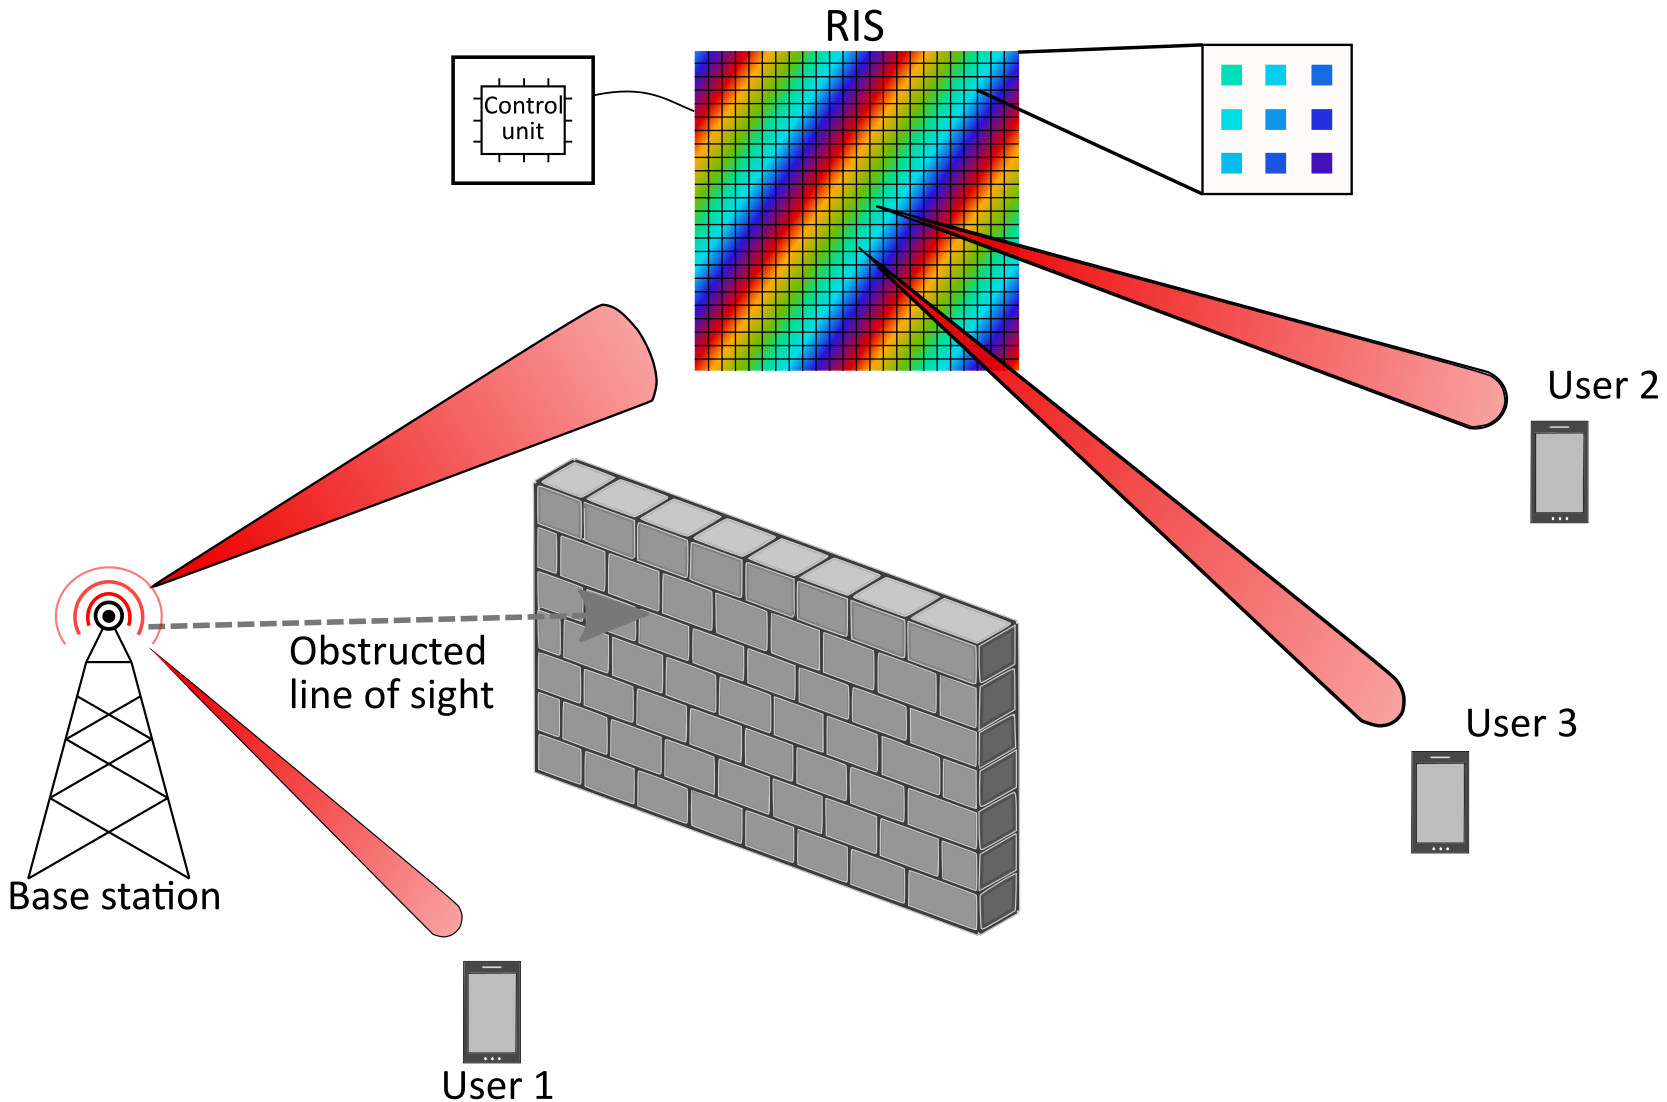
\includegraphics[width=0.96\columnwidth]{Figures/Motivation.png}
	\caption{Example scenario where a \gls{RIS} establishes a link between a transmitter and two receivers despite an obstacle blocking the \gls{LOS} path.}
	\label{fig:RISScenario}
\end{figure}

% Introducing LC crystals
    So far, various \gls{RIS} prototypes have been reported in the literature, which mainly employ \gls{SC} technologies (e.g., \gls{PIN} diodes \cite{tang2020wireless}, varactors \cite{alamzadeh2021reconfigurable}, % conference
    \gls{RF} switches \cite{rossanese2022designing}) to realize the phase shifts. Although a feasible choice of design, their cost and resolution (in case of \gls{PIN} diodes) can be prohibitive in building truly large and cost-efficient large \glspl{RIS}. An alternative to these technologies is \gls{NLC} technology. In the last two decades, \glspl{NLC} have been studied for the microwave, \gls{mm-Wave}, and THz frequency bands \cite[Ch. 5]{ferrari2022reconfigurable}. %\red{\cite{weickhmann2017liquid}}. 
    If fabrication in standard \gls{LCD} technology is adopted, the manufacturing cost of \gls{NLC}-\glspl{RIS} will be reduced to that of a commercial \gls{LCD} television. Hence, \gls{NLC}-based designs have the advantages of cost-effective scalability, low energy consumption, and continuous phase shifting, which make them a suitable candidate for realizing extremely large passive \glspl{RIS}. Despite these attractive features, \gls{NLC} characteristics impose new challenges when being integrated into today's mobile communication systems, most notably due to their slow tuning capabilities as compared with \gls{SC}-\glspl{RIS}.

% Contributions of this paper:
In this article, we aim at bridging the gap between microwave and antenna design aspects of \gls{NLC}-\glspl{RIS} with mobile communication aspects. To this end, we first review the basic physical principles of LC theory and introduce two different realizations of \gls{NLC}-\glspl{RIS}, namely the \gls{RA} and \gls{PA} methods. Thereby, we particularly highlight their key physical and hardware properties that have a direct impact on the system design and RIS reconfiguration strategy. This is complemented by a concrete comparison against the alternative technologies for building RISs (i.e., \glspl{SC} and \gls{MEMS})  in terms of feasibility, cost, power consumption, reconfiguration speed, and bandwidth. Finally, we delve into the challenges of \gls{NLC}-\glspl{RIS} (slow response time, temperature dependencies, bandwidth) and present potential directions for both theoretical and experimental research in order to overcome these challenges.




% Basic path loss and phase gradients needed assuming far-field ozdogan2019intelligent

% \begin{itemize}
%     \item RISs have been the subject of extensive investigations in the past few years, esp in the context of 6G communications. 
%     \item then what are RISs... 
%     \item advantage and disadvantage --> Perhaps the cost and HW complexity can be listed as a disadvantage. --> This puts their practicality under question. and determines whether they will be used as a widely deployed technology or as a specialized high-end gadget limited to a few use cases.  
%     \item in this article, we provide an overview on what is the state of the art on RIS design. Bringing together the knowledge from antenna design and communication systems, we shed light on alternative technologies which allow scalable and effective RIS manufacturing and operations. 
% \end{itemize}

% Introduction

% In recent years, there has been considerable interest in \glspl{RIS}, particularly within the context of 6G communications. 
% The potential for significant improvements in communication and sensing capabilities through the use of large, passive tunable reflectors has led to the development of models and subsequent attention from the microwave community towards the practical implementation of \glspl{RIS}~\cite{kazim2020wireless}.

% \glspl{RIS} have been the subject of extensive investigations in the past few years, especially in the context of 6G communications. With the development of models predicting massive communication and sensing improvements through large, passive (from the \gls{RF} perspective) tunable reflectors, the attention of the \gls{RF} community has been brought towards the realization of such \glspl{RIS} }. 
%Tests include the enhancement of the wireless communications in rich scattering channels \cite{alexandropoulos2021reconfigurable}. % Missing some additional sentence

% What is a RIS and typical scenario
% \glspl{RIS} are planar electromagnetic surfaces comprised of many independently tunable reflecting elements. 
% These reflecting elements can be adjusted externally to modify the phase and, in certain instances, the amplitude of the signal reflected at each element \cite{venkatesh2022programmable}. 
% Through the superposition of reflections from each element, the reflection pattern can be dynamically tuned, eliminating the need for complex decoding, encoding, and processing operations. 
% While demonstrations of tunable surfaces for beam switching purposes dates back to 1995 in the antennas and propagation society \cite{javor1995design}, their large scale application to mobile network has only been recently considered.

% Essentially, an \gls{RIS} functions as a tunable reflectarray without a fixed, known feeding antenna located close to the reflectarray. This property can be leveraged in wireless networks to spatially focus the signal from the transmitter to the receiver, thus increasing the received power as illustrated in Figure \ref{fig:RISScenario}. 
% From a radio frequency (RF) perspective, an \gls{RIS} is significantly less complex than traditional relays due to its passive nature, i.e., lacking the typical RF processing chain (dedicated amplifiers, filters, oscillators, mixers...). 
% However, this passive nature also means that \glspl{RIS} cannot actively amplify the signal and thus, they must have very large apertures to collect and focus enough of the desired signal toward the receiver \cite{bjornson2019intelligent}. 


% \glspl{RIS} are planar electromagnetic surfaces consisting of a large number of independently tunable reflecting elements. Depending on the design, each reflecting element can be externally tuned to alter the phase and, in some cases, the amplitude of the signal reflected at each reflecting element \cite{venkatesh2022programmable}. Due to the spatial superposition of the reflections of each element, the reflection pattern can be dynamically tuned without complex decoding, encoding, and \gls{RF} processing operations. Such a \gls{RIS} can therefore be seen as a tunable reflectarray without a fixed, known feeding antenna placed close to the reflectarray.

% In a wireless scenario, one or multiple transmitters and receivers can be distributed at random positions, and the \gls{RIS} should be able to enhance the performance by dynamically redirecting the power from one or several transmitters to one or several receivers, achieving an increased received power by spatially focusing the signal from the transmitter to the receiver as depicted in Fig. \ref{fig:RISScenario}.



% Difference to relays and why we need large RIS and need for considering radiating near field
% From the system perspective, a \gls{RIS} can be understood as a relay that lacks dedicated filters, oscillators, and mixers to demodulate the signal, as well as amplifiers to increase the power retransmitted.
% Therefore, its hardware is substantially simpler than other relay techniques, especially at higher operating frequencies \cite{pan2021reconfigurable}.
% This limitation of the capabilities of a \gls{RIS} to \textit{bundling} the energy from a transmitted signal more efficiently towards the receiver by spatially focusing it means that large \glspl{RIS} are needed to substantially increase the received power at the receiver.
% To receive and also improve the angular resolution of a \gls{RIS}, the realization of large panels with at least hundreds of elements is envisioned, since \glspl{RIS} with lower number of elements would be outperformed by decode-and-forward relays with comparably simpler and electrically smaller antenna modules \cite{bjornson2019intelligent}. 
%\sout{The large size of \glspl{RIS} also results in the fact that the far-field approximation of $d_{ff} > 2D^2/\lambda_0$ is not always fulfilled, being $\lambda_0$ the wavelength in vacuum at the operating frequency. 
%When the far-field approximation is not fulfilled, the \gls{RIS} is large and close enough to a certain point that it can focus the signal at a certain point. It therefore acts as a lens and the free space path loss of $1/(4 \pi R^2)$ does not hold, i.e., can be overcome. %When the far-field approximation is not fulfilled, the often assumed linear phase progression between radiating elements is not the optimal solution for maximum received power at the receiver, i.e., the \gls{RIS} should be configured so that its focal point is not at an infinite distance away from it, but at a finite distance. 
%Such region of space receives the name of radiating near-field and can hold for the transmitter position, the receiver position, or both, increasing the amount of information needed to configure the optimum phase distribution for maximum \gls{SNR} \todo{SINR?} \cite{bjornson2020reconfigurable}.
%The only \textit{cost} of operating in it is that not only the angle, but also the distance between the \gls{RIS} and the focal point need to be known to calculate the required phase distribution at the \gls{RIS}.}


% \ara{Here we talk about the move towards exp prototypes... }

% In recent years, we have observed a surge in efforts to prototype and build \glspl{RIS}. The majority of these existing prototypes use semiconductors (e.g., \gls{PIN} diodes, varactors, RF-switches) to realize the phase shifts. \ara{@AJS:Is there something with mems?}Although a feasible choice of design, their cost and their resolution (in case of \gls{PIN} diodes) can be prohibitive in building truly large and cost-efficient large \glspl{RIS}. An alternative to these technologies is \gls{NLC}-based design. In the last two decades, \glspl{NLC} have been studied  for the microwave, \gls{mm-Wave}, and THz frequency ranges \cite{ferrari2022reconfigurable}, \cite{weickhmann2017liquid}. If fabrication in standard \gls{LCD} technology is adopted for \gls{NLC}-based \glspl{RIS}, the asymptotic cost of \gls{NLC}-based RIS will reduce to that of a commercial LCD television. While \gls{NLC}-based design have the advantage of lower cost, lower energy and continuous phase shifting, their tuning time\footnote{The time it takes for the phase shifters to move from one configuration to the other.} is higher than semiconductor-based RIS. Despite their attractive properties and high potential, \gls{NLC} characteristics also impose challenges to today's communication which are, for instance. designed for fast tuning of semiconductor-based phased arrays. 

% In this article, we aim at bridging the gap between microwave and antenna design aspects of RIS with mobile communication aspects. Specifically, we elaborate on technical details of \gls{NLC}-based RIS design. This is complemented by a concrete comparison against the alternative technologies for building RISs (i.e., semiconductors and \gls{MEMS}). Finally, we delve into challenges of \gls{NLC}-based RIS (slow response time, temperature dependencies, bandwidth) and potential pathways for overcoming those challenge (e.g, transition-aware beamforming), %designfor large quantities of large panels could become considerably low.
%This would make \glspl{NLC} an enabler technology for large \glspl{RIS}, e.g., 40 to 80 inch (ca. 2 m) diagonals, as current commercial televisions. However, despite the low-cost and their low-energy consumption 

%\sout{In this article, we discuss the potential of \gls{NLC}-based \glspl{RIS} and provide a short overview of possible alternative technologies. Finally, we discuss the current challenges of \gls{NLC}-\glspl{RIS} to be practically deployed in 6G networks.}
% Main criteria for the wide use of RISs in 6G
% One of the main factors currently limiting the widespread use of \glspl{RIS} is the lack of large, cost-efficient, reconfigurable structures.
% This publication introduces the use of \gls{NLC} as a suitable technology to enable \glspl{RIS} with such properties. 
% This information aims to guide future research and developments in the field of \gls{NLC}-based \glspl{RIS} by analyzing the potential as well as the limitations of this technology for different applications, bringing together the knowledge from antenna design and communications systems. 

% \sout{This publication starts with a brief introduction of the competing techniques based on \gls{PIN} diodes and \gls{MEMS}. 
% Afterwards, the Microwave \gls{NLC} technology is introduced. 
% It continues with the analysis of two different unit cell configurations, followed by a general overview of the challenges of \gls{NLC} technology.
% Finally, %given the introduced advantages and disadvantages, 
% potential applications of \gls{NLC} \glspl{RIS} are introduced.}




\section{Liquid Crystal-based RISs}

In this section, we first present the basic operating principles of \gls{NLC} technologies. Subsequently, we introduce two of the existing \gls{NLC}-\gls{RIS} implementations, as well as the hardware components required for implementing them.

\subsection{Basic physical principles of LC technology}\label{Sec:Basic}

\textbf{Phase shifting capability:}  
The working principle of \gls{NLC} is based on its electromagnetic anisotropy\footnote{\gls{NLC} molecules exhibit different electromagnetic properties depending on their relative orientation with the \gls{RF} electric field.}. In particular, due to the ellipsoidal shape of \gls{NLC} molecules, the \gls{NLC} presents a larger permittivity (i.e., higher phase shift) when the electric field, $\vec{E}_{\rm RF}$, is aligned with the major axis of the molecules, $\vec{n}$, than when it is aligned with  the minor axis (i.e., lower phase shift), see~Fig.~\ref{fig:LCmolres}. Therefore, by controlling the orientation of \gls{NLC} molecules, we can alter the phase shift of the \gls{RF} signals. 

 % \subfloat[]{
 %        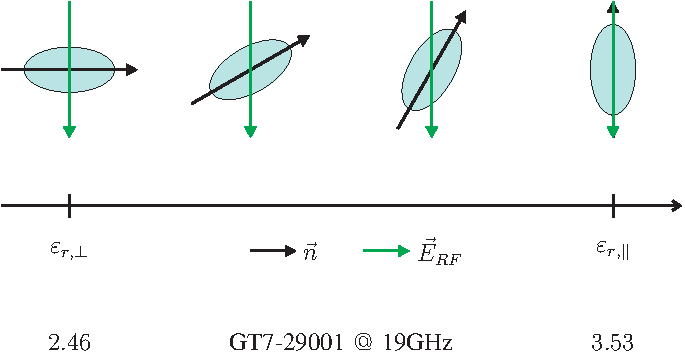
\includegraphics[width=0.7\columnwidth]{Figures/LCmolecules.pdf}
 %        \label{fig:LCmoledulces}
 %    }\hfill
	% \subfloat[]{
	% 	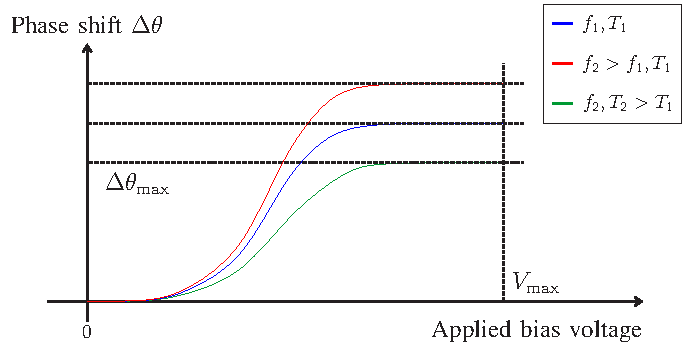
\includegraphics[width=0.8\columnwidth]{Figures/LCresponse.pdf}
	% 	\label{fig:LCresponse}
 %    }
    


%To exploit the above feature of \glspl{NLC}, the orientation of the LC molecules should be changed in a controlled manner.  

This is achieved by placing a thin \gls{NLC}-layer between two electrodes. Thereby, when no voltage is applied, the molecules are in their relaxed phase, where $\vec{E}_{\rm RF}$ is perpendicular to $\vec{n}$, and hence \gls{NLC} shows a minimum permittivity $\varepsilon_{r,\perp}$. In contrast, when the maximum voltage is applied, the \gls{NLC} molecules orient along the induced external electric field, which leads to $\vec{E}_{\rm RF}$ being now parallel to $\vec{n}$ and hence a maximum permittivity of $\varepsilon_{r,\parallel}$. The maximum achievable phase shift, $\Delta\theta_{\max}$, therefore scales with $\Delta\varepsilon = {\varepsilon_{r, \parallel}} - {\varepsilon_{r, \perp}}$.  The \gls{NLC}-layer permittivity and the corresponding maximum achievable phase-shift are dependent on the operating frequency as well as temperature, cf. Fig.~\ref{fig:LCmolres}, which will be elaborated further in Section~\ref{sc:challenges}. 

\textbf{Response time:} The alignment of the \gls{NLC} along the electrodes when applying a voltage (for positive phase shifts) is faster than the alignment of the molecules due to mechanical anchoring forces (for negative phase shifts). For this reason, usually the latter slow transition is considered and modelled by the decay or switch-off response time, $\tau_{\rm off}$, which is proportional to $\tau_{\rm off} \propto {\gamma_{\rm rot}{d_{\rm LC}^2}}/{K_{11}}$,  where  $\gamma_{\rm rot}$ is the rotational viscosity, $d_{\rm LC}$ is the \gls{NLC}-layer thickness, and $K_{11}$ is the splay deformation factor of the \gls{NLC}. Therefore, the response time can be reduced by adopting a narrower \gls{NLC} layer; however, this implies more delicate (hence costly) manufacturing and higher conductor losses, motivating research to reduce losses in thin phase shifters \cite{neuder2023compact}.  The \gls{NLC} thickness, $d_{\rm LC}$, can be as low as a few \SI{}{\micro\meter} for switch-off response times, $\tau_\mathrm{\rm off}$, in the order of tens of milliseconds. 

\begin{figure}[t]
	\centering
 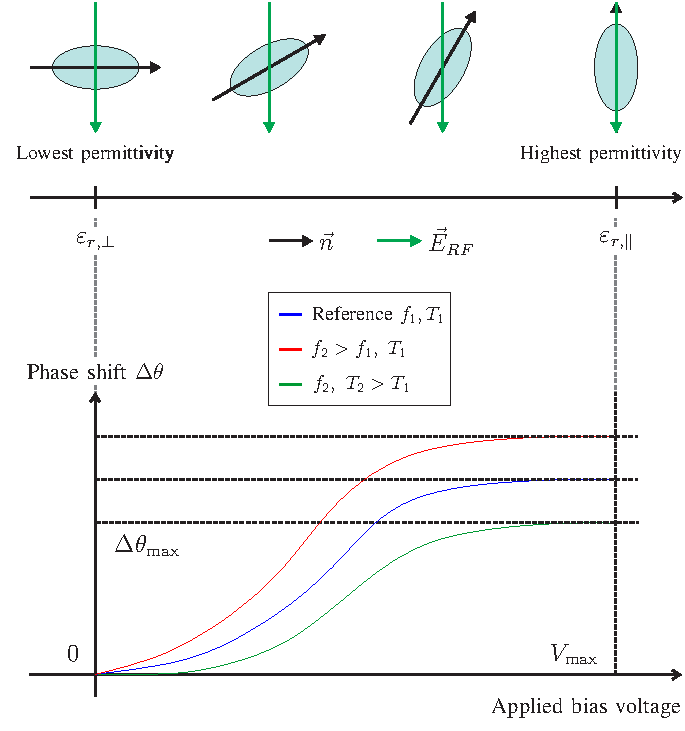
\includegraphics[width=0.8\columnwidth]{Figures/LCmolres.pdf}
	\caption{Top figure: Observed \gls{NLC} permittivity depending on the orientation between the \gls{RF} electric field, $\vec{E}_{RF}$, and the \gls{NLC} molecule major axis, $\vec{n}$. The lowest permittivity, $\varepsilon_{r,\perp}$, is observed when $\vec{E}_{RF}$ and $\vec{n}$ are orthogonal while the highest permittivity, $\varepsilon_{r,\parallel}$, is observed when $\vec{E}_{RF}$ and $\vec{n}$ are parallel to each other. Bottom figure: Schematic illustration of the corresponding phase shift achieved by applying bias voltage leading to the change in permittivities. This figure illustrates that the achievable phase shift depends on the operating frequency $f$ and temperature $T$.}
 		\label{fig:LCmolres}
\end{figure}

% \begin{figure*}[t]
% 	\centering
% \subfloat[]{
%         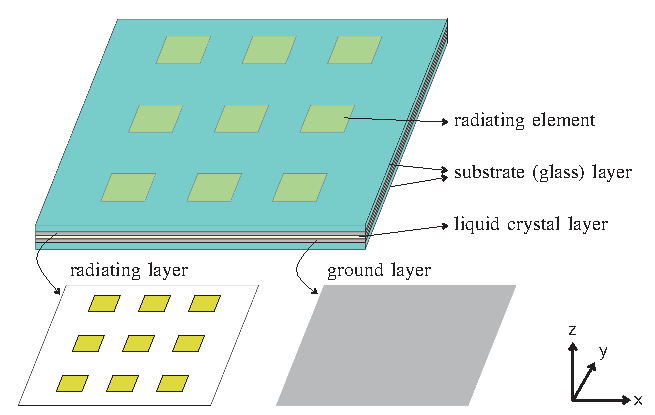
\includegraphics[width=0.8\columnwidth]{Figures/LCrisRA.pdf}
%         \label{fig:LCrisRA}
%     }\hskip 1cm
%     \subfloat[]{
%         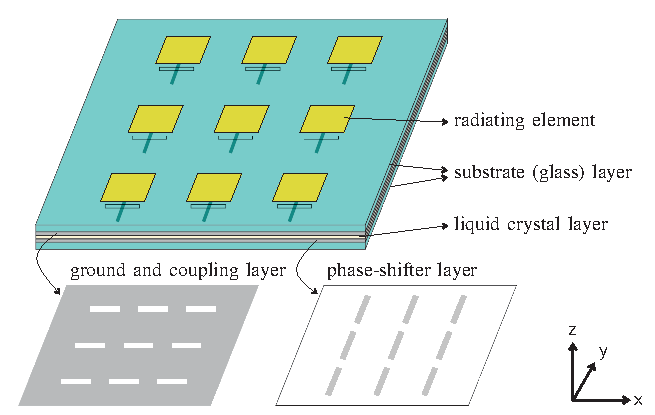
\includegraphics[width=0.8\columnwidth]{Figures/LCrisPA.pdf}
%         \label{fig:LCrisPA}
%     }\hfill
% 	\subfloat[]{
% 		\includegraphics[width=0.95\columnwidth]
%   {Figures/LCunitRA.pdf}
% 		\label{fig:LCunitRA}
%     } \hskip 0.1cm
%     \subfloat[]{
% 		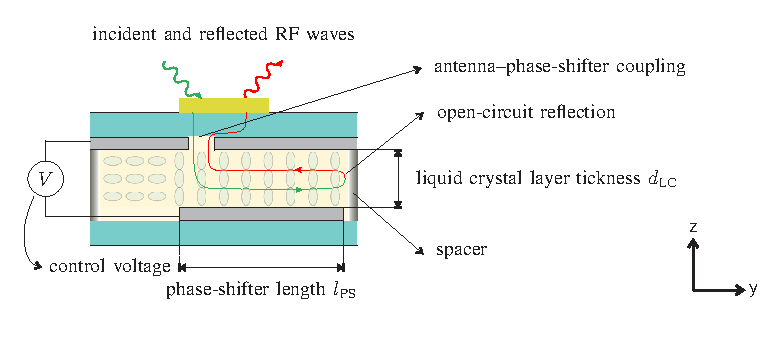
\includegraphics[width=0.95\columnwidth]{Figures/LCunitPA.pdf}
% 		\label{fig:LCunitPA}
%     } 
%     \caption{Schematic illustration of reflect-array (left-hand side) vs. phased-array (right-hand side) LC-based RISs. The top figures illustrate the implementation of LC-based RISs in three dimensions  whereas the bottom figures show a single unit cell from $\mathsf{y}-\mathsf{z}$ cross-section. The different layers, propagation path of the RF wave, and important design parameters such as phase-shifter length $l_{\rm PS}$ (influencing the maximum phase-shift and insertion loss) and LC layer thickness $d_{\rm LC}$ (impacting the RIS response time) are schematically illustrated.}
%     \label{fig:LCris}
% \end{figure*}

\begin{figure*}[t]
	\centering
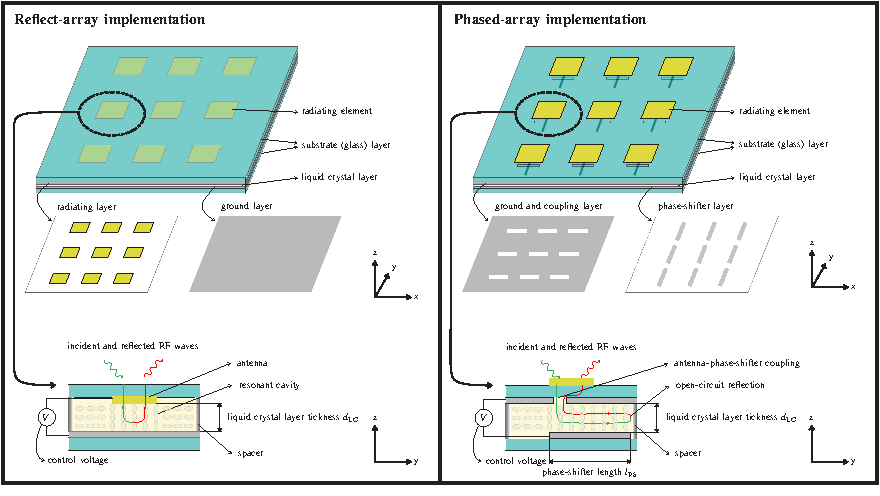
\includegraphics[width=1.9\columnwidth]{Figures/LCrisPARA.pdf}
    \caption{Schematic illustration of reflect-array vs. phased-array LC-RISs. The top figures illustrate the implementation of LC-RISs in three dimensions whereas the bottom figures show a single unit cell from $\mathsf{y}-\mathsf{z}$ cross-section. The different layers, propagation path of the RF wave, and important design parameters such as phase-shifter length $l_{\rm PS}$ (influencing the maximum phase-shift and insertion loss) and LC-layer thickness $d_{\rm LC}$ (impacting the RIS response time) are schematically illustrated.}
    \label{fig:LCrisPARA}
\end{figure*}

\textbf{Insertion loss:} The interaction of the \gls{RF} wave with the \gls{RIS} circuit introduces a certain insertion loss, $L_{\rm ins}$, which depends on the design as well as material properties such as dielectric losses, $\tan\delta$, and conductor losses. For the \gls{PA} implementation (see Section~\ref{sec:RISimplementation}), the phase-shifter length $l_{\rm PS}$ has a direct impact on the final insertion loss and maximum phase shift, see Fig.~\ref{fig:LCrisPARA}. In fact, increasing the phase-shifter length yields a higher maximum phase shift $\Delta\theta_{\max}\propto l_{\rm PS}$ at the cost of a larger insertion loss $L_{\rm ins} \propto l_{\rm PS}$. 

\textbf{Clearing point temperature:} Another physical property of \glspl{NLC} is the temperature at which an \gls{NLC} phase is converted to an isotropic liquid.  This temperature is known as the clearing point, $T_c$, after which tunability is no longer possible, and hence constitutes the highest operation temperatures. 
From the material design perspective, the main targets of \gls{NLC} design is to achieve high phase-shift contrasts, $\Delta\varepsilon $, low dielectric losses, $\tan\delta$, high clearing point temperatures, $T_c$,  and fast response times by reducing the rotational viscosity of the molecules, $\gamma_{\rm rot}$. 
The values of these parameters for several commercially available \gls{NLC} mixtures are shown in Tab.~\ref{tab:LCtypes}.

\begin{table*}
\centering
\caption{LCs for mm and sub-mm wave bands and their material properties. \cite{jakoby2020microwave}}
\label{tab:LCtypes}
\begin{tabular}{@{}lcccccccc@{}} \toprule
LC        & $\varepsilon_{r,\perp}$ & $\tan\delta_\perp$ & $\varepsilon_{r,\parallel}$ & $\tan\delta_\parallel$ & {$\Delta \varepsilon$} & $T_c (^\circ \text{C})$&  $K_{11} (\text{pN})$  &  $\gamma_{\rm rot} (\text{Pa} \cdot \text{s})$ \\ \midrule %& Ref.  &    \cite{manabe2013liquid}  &    \cite{fritzsch201977} &    \cite{weickhmann2017liquid}  &    \cite{fritzsch201977} 
K15 (5CB) & 2.7                     & 0.0273            & 3.1                         & 0.0132                & 0.4                  & 38.0            &    7.0          & 0.126                          \\
GT3-23001 & 2.41                    & 0.0141            & 3.18                        & 0.0037                & 0.77                 & 173.5           &    24           & 0.727                          \\
GT5-28004 & 2.40                    & 0.0043            & 3.32                        & 0.0014                & 0.92                 & 151.0           &    11.8         & 5.953                          \\
GT7-29001 & 2.46                    & 0.0116            & 3.53                        & 0.0064                & 1.07                 & 124.0           &    14.5         & 0.307                        \\ \bottomrule
\end{tabular}
\end{table*}

\subsection{LC-based RIS implementation} \label{sec:RISimplementation}

Next, we first discuss the basic components that are required to realize an \gls{NLC}-\gls{RIS}. Subsequently, we introduce two implementation approaches of \gls{NLC}-\glspl{RIS}, namely the \gls{RA} and \gls{PA} methods, and discuss their advantages and limitations. Both implementations are potentially compatible with current \gls{LCD} technology, which is a great advantage for the realization of cost-effective large \glspl{RIS}, see Fig.~\ref{fig:LCrisPARA}.


\textbf{Basic components:}  The thin \gls{NLC} layer is usually placed between two layers of glass. 
The choice of glass over more common materials is due to the fact that a very thin \gls{NLC} layer with a well-defined thickness needs to be achieved over large panels, therefore a stiff, smooth solid substrate is needed.
Due to its liquid state, solid spacers are needed to maintain the desired \gls{NLC} layer thickness. 
Moreover, the circuits of planar \gls{NLC} are commonly grown directly on glass substrates. Thereby, one or both sides of each glass are selectively metalized to pattern the desired circuitry, e.g., control lines and biasing electrodes. In particular, one of the glass substrates is often metalized to act as a ground layer for biasing all unit cells, whereas the other glass is selectively metalized for introducing phase-shifting control voltage of individual unit cells, see Fig. \ref{fig:LCrisPARA}. 
To receive and re-radiate the phase-shifted signal, a radiating element is needed, usually a patch or a dipole antenna. 





% Patch antenna and coupling slot
%Finally, to couple the phase shifter with free space and to be able to receive and reradiate the phase-shifted signal, a radiating element is needed. 
%This radiating element is often e.g. a patch or a dipole antenna.
%slot-coupled patch antenna so that the patch is coupled to the phase shifter on the opposite side of the ground, and the effect of tuning \gls{NLC} mainly affects the phase shifter, but not the antenna as presented in \cite{strunck2013continuously} and sketched in Fig. \ref{fig:method_PhasedArray}.

\textbf{Reflect-array implementation:} In this method, there is a common ground for all \gls{RIS} elements and the \gls{NLC} layer is directly between the antenna (acting also as one of the biasing electrodes) and the ground, see Fig. \ref{fig:LCrisPARA}. This structure forms a resonant cavity between the metal patch and the uniform ground plane. The advantage of this design is its simplicity since no patterning of the ground plane is necessary and therefore only the layer with the patches must be etched. This avoids any alignment issues during assembly. However, the limitations of this method are: \textit{i)} 
Due to the resonant effect, there is a limited bandwidth at which a nearly constant group delay and low amplitude
variations can be achieved. 
\textit{ii)} Thicker LC layers, $d_{\rm LC}$, are needed to support wideband
resonances with a low radiation quality factor to minimize
the losses. This results in slow response times, {$\tau_{\rm off}\geq 10$s}.
\textit{iii)} The LC biasing lines are comprised in the same layer of the patches and therefore need to be considered in its design.
As a guiding value, such designs achieve impedance bandwidths\footnote{The range of frequencies over which the antenna has an acceptable (-10 dB) impedance matching.} below 10\% and insertion losses in the range 6 to 10 dB.

\textbf{Phased-array implementation:} In this method, one of the glass substrates is metalized such that each \gls{RIS} element has a dedicated phase shifter (i.e., a biasing electrode). Moreover, the ground layer is patterned to couple the radiating elements to the phase-shifters, see Fig. \ref{fig:LCrisPARA}. For the realization of the phase shifters, transmission line topologies compatible with \gls{LCD} manufacturing are needed.
One of these transmission lines is the \gls{IMSL} which is depicted in Fig.~\ref{fig:LCrisPARA}. 
The transmission line should be terminated with a reflective end. % which can be achieved via an open or a short-circuit at the end of the phase shifter. For a conventional \gls{IMSL}, an \gls{RF} short circuit can be achieved by connecting the phase-sifter end to the ground, but this would also short-circuit the voltage applied for biasing. Furthermore, the realization of bias through glass compatible with mass production and very thin \gls{NLC} layers, $d_{\rm LC}< $\SI{10}{\micro\meter} remains a challenge. 
A suitable solution is the abrupt termination of the metal strip in an open end. 
Although such an open-end shows increased undesired radiation, this radiation is mainly proportional to the thickness of the \gls{NLC} layer, $d_{\rm LC}$. 
Small $d_{\rm LC} <\ $\SI{100}{\micro\meter} hence minimizes this effect.
The advantages of the \gls{PA} method are: \textit{i)} bandwidth is not limited by the phase shifter, and a thick glass in the radiating layer allows a wideband radiating element. A nearly constant group delay and low amplitude variations across the bandwidth can be achieved. 
\textit{ii)} Thin \gls{NLC} layers, $d_{\rm LC}$, are possible and lead to response times, $\tau_{\rm off}<100$~ms.
\textit{iii)} The LC biasing lines are comprised in an additional layer. They do not disturb radiation, but additional processing steps are needed to metalize and pattern the additional layer. The insertion loss of the phase shifter for thin $d_{\rm LC}$, specifically \SI{4.6}{\micro\meter}, is determined to be \SI{4.5}{\dB} for full \SI{360}{\degree} tunability at \SI{28}{\GHz} in~\cite{neuder2023compact}. The matched impedance bandwidth is expected to range around \SI{15}{\percent}. 
%Another advantage of thin layers for large surfaces is the amount of \gls{NLC} needed. Assuming \SI{100}{\micro\meter} and \SI{4.6}{\micro\meter} thicknesses for \gls{RA} and \gls{PA}, respectively, an \gls{RIS} would need $21.6$ times less \gls{NLC} for the \gls{PA} method. Even when acquiring high \gls{NLC} amounts, this difference can notably reduce the material cost. 

% Given the separation of phase shifting and the radiating layer in phased-array implementation, the thickness of glass substrate and the LC layer are indepedent. This allows to use very thin LC layers (e.g., a few µm) which reduces tuning time while having a thicker glass substrate (e.g., \ara{@AJS: can u provide a scale, a few hundred micrometer?}) which increases the bandwidth. %to  thickness in the radiating layer, which is desired to be electrically thick for large bandwidth. 
% As a result, response times as fast as tens of ms can be achieved while exhibiting large impedance bandwidth\ara{@AJS: can we say 8\%?}. The insertion loss of the phase shifter for thin $d_{\rm LC}$, specifically \SI{4.6}{\micro\meter}, is determined to be \SI{4.5}{\dB} for full \SI{360}{\degree} tunability at \SI{28}{\GHz} in~\cite{neuder2023compact}. The matched impedance bandwidth is expected to range around \SI{15}{\percent}.\vahid{Can we report impedance bandwidth and insertion loss to mirror the reflect-array method?} \alejandro{@Robin: include your achieved insertion loss values for the phase shifter, as well as expected RIS bandwidths (with radiations). 2-4 sentences to clarify difference between phase shifter and radiation element if needed.}

%A final advantage of thin layers for large surfaces is the amount of LC needed. Assuming \SI{100}{\micro\meter} and \SI{4.6}{\micro\meter} thicknesses, an \gls{RIS} would need $21.6$ times less \gls{NLC} for the phased array method. For example, $2 \times 2\ m$ \gls{RIS} would need \SI{400}{\milli \liter} and \SI{18.4}{\milli\liter}, respectively.
%Even when acquiring high \gls{NLC} amounts, this difference can notably reduce the material cost. 

%Similarly, patterning the ground plane helps improve the performance, but at the cost of an additional (3rd) selectively metalized layer.

% % Reflection - half length of phase shifter needed
% \vahid{@Alejandro: Is this paragraph valid only for phased-array implementation?} 
% \alejandro{Yes, the termination is only for phased-array implementation.}
% An important difference between the transmission-type phase shifters {\color{red} used in LCD technologies} and the reflection-type phase shifters needed for the 
%  \gls{RIS} is that the latter needs to be terminated with a reflective end. 
% This can be achieved via an open or a short-circuit at the end of the phase shifter. 
% For a conventional \gls{IMSL}, an \gls{RF} short circuit can be achieved by connecting the phase-sifter end to the ground, but this would also short-circuit the voltage applied for biasing. 
% Furthermore, the realization of bias through glass compatible with mass production and very thin \gls{NLC} layers, $d_{\rm LC}< $\SI{10}{\micro\meter} remains a challenge. 
% A viable solution is the abrupt termination of the metal strip in an open end. 
% Although such an open-end shows increased undesired radiation, this radiation is mainly proportional to the thickness of the \gls{NLC} layer, $d_{\rm LC}$. 
% Low $d_{\rm LC} <\ $\SI{100}{\micro\meter} hence minimizes this effect.  
% %Notice that a larger thickness and relative permittivity of the bottom substrate, $d_b$ and $\varepsilon_{r,b}$, also increase the radiation of the open-ended transmission line. % I am talking about the IMSL. Specify it?
% The advantage of operating the phase shifter in reflection is that the signal travels twice through it, so that the required length for a full \SI{360}{\degree} is halved compared to traditional transmission-type phase shifters for phased antenna array solutions.

% \subsection{Existing LC-based RIS experimental work}

% Recently, a few publications have shown the use of \gls{NLC} for the realization of digital metasurfaces \cite{ma2022digital}. For instance,
% \cite{wu2020liquid} presents the realization of an LC-based reflective \gls{RIS} with 1-bit programmable elements. 
% Similarly, a 1-bit design at \SI{0.645}{\tera\hertz} is presented in \cite{fu2022flexible} for transmissive RISs.  In this case, 1-bit, two-column-wise biasing is realized, so that an array of $64\times64\ $elements is controlled with 32 electrodes and the ground plane as a common electrode. The designs in \cite{wu2020liquid,fu2022flexible} follow the reflectarray implementation. In \cite{neuder2023compact}, initial works for realizing an LC-based RIS following the phased-array implementation have been reported. \alejandro{We could remove 1 or 2 references here if we have too many.}
% \ara{@AJS: I didn't get why these LC works on 1 bit and ours isn't... because in the advantages in the paragraph below we do mention continuous phase shifting as a merit}
%Differently than the design shown in Fig. \ref{fig:method_Reflectarray}, which consisted of an etched metal layer over a homogeneous ground plane, \cite{liu2021programmable} presents a \gls{NLC} metasurface which needs two patterned metallic layers to function. 
%\vahid{This reference is yet a new architecture than those in Fig.~\ref{fig:LCris} and could distract the reader. Shall we remove it? We have anyway only 15 references to cite.}
%\alejandro{Then I agree - I do not think it should be a priority.}





%Include Figure of the patch and the slot here



\section{Comparison of Technologies for Building \glspl{RIS}}
From a broad perspective, there are three main technologies for realizing a \gls{RIS}, namely \gls{NLC}, \gls{SC}, and \gls{MEMS}. In this section, we provide an overview of each method and discuss the respective advantages and limitations. 


\begin{table*}
\centering
\caption{Comparison of Technologies used for the Realization of RIS.}\label{tab:comparison}
\begin{tabular}{llcccc}
\hline
                  & Varactor                                 & PIN Diode                                & \gls{MEMS} Switch                 & \gls{MEMS} Mirror                  & LC                                                            \\ \hline
Tuning time       & ns                                       & ns                                       & $\mathrm{\mu s}$                                        &$\mathrm{100s \: of \: \mu s}$                                     & $>$ 10 ms                                                      \\
Tunability        & continuous                               & discrete (1 bit/diode)                   & discrete                                       & discrete                                            & continuous                                                    \\
Power consumption & medium                                   & medium                                   & low                                            & low                                                 & low                                                           \\
Scalability       & low (cost per diode)                     & low (cost per diode)                     & medium (encapsulation)                          & medium (cost per area)                              & high                                                          \\
Frequency range   & few GHz                                  & mm-Wave                                  & mm-Wave                                        & THz                                                 & $>$ 10 GHz                                                    \\
Cost              & high                                     & high                                     & high                                           & high                                                & low                                                           \\
Example           & \cite{tawk2012varactor} & \cite{tang2020wireless} & \cite{ferrari2022reconfigurable}, Ch. 4 & \cite{schmitt20213} & \cite{neuder2023compact, karabey20122} \\ \hline
\end{tabular}
\end{table*}


\subsection{\gls{NLC}-based \glspl{RIS}}
The fundamentals of \gls{NLC}-\glspl{RIS} have been discussed in detail in the previous section, hence we elaborate on the advantages and limitations of this technology. 

{\bf Advantages:} 
One of the key merits of \gls{NLC}-\glspl{RIS} is {\it scalability at low-cost}. \gls{NLC} has been used for standard \gls{LCD} fabrication processes for decades. 
Therefore, the production of large \gls{NLC} panels is technologically both very accessible and inexpensive. 
The cost of \gls{NLC}-\glspl{RIS} can be even less than \gls{LCD} displays due to the lower number of \textit{pixels}, the lack of backlight, as well as the larger tolerances compared to, for example, the strict color accuracy standards applied to displays. %To date, several start-ups are already working towards the production of \gls{NLC}-based antenna\footnote{Kymeta Corp: https://www.kymetacorp.com}. 
The other advantage of \gls{NLC} is its {\it low power consumption}.
Due to its dielectric nature, \gls{NLC} experiences minimal current flow only to alter its state, specifically for rotating the LC molecules. Nonetheless, this power requirement is significantly lower compared to other technologies such as \gls{PIN} diodes. 
The other important feature of \gls{NLC} is the {\it continuous tuning} capability, which is useful when sophisticated wavefront shaping (beyond a simple narrow reflection beam) is required, e.g., to reduce interference in multi-user systems.
%\sout{The response of the \gls{NLC} can be continuously tuned between its two extreme states, parallel and orthogonal. In the planar structures introduced in Section \ref{sc:LCRIS}, this is achieved by applying a voltage between \SI{0}{\volt} for the unbiased state, and $V_{max}$ for the fully biased states. Using common \glspl{DAC}, this can be achieved with resolutions of \SIrange{12}{16}{\bit}, achieving a quasi-continuous transition between both states. Furthermore, \gls{NLC} shows negligible hysteresis, so that a direct mapping between voltage applied and phase response is possible without considering the previous states. This technique is possible for both the reflectarray and the phased array methods, although the former often suffers from stronger amplitude variations for the different biasing states. }

{\bf Limitations:} Despite major advances in \gls{NLC} microwave community, the response time of these devices are still higher than \gls{SC} and \gls{MEMS} (e.g., $>10$~ms for \gls{PA} and {$>10$~s} for \gls{RA}). This implies that while the \glspl{RIS} are able to adapt to the user movement (e.g., on the order of seconds), they cannot adapt to fast fading. In addition, \gls{NLC}-\glspl{RIS} are suitable mainly for high frequencies $>10\ $GHz and cannot be adopted for  sub-$6$~GHz communication systems featuring rich multi-path environments. Moreover, the phase-shifting behavior of \gls{NLC}-\glspl{RIS} is temperature-dependent, see Fig.~\ref{fig:LCmolres}, which necessitates the adaption of reconfiguration strategy for the environments with significant temperature variations, see Section~\ref{sec:temperature} for possible solutions. 
%Potential reference if we want to highlight the potential of glass manufacturing without going into detail \cite{chaloun2023rf}.

\subsection{\gls{SC}-based \gls{RIS}}
\glspl{SC} are very common for \gls{PA} antennas. Similar  designs have been leveraged in prototyping \glspl{RIS}. Under this category, there are two common approaches, namely \gls{PIN} diodes and varactors. %\alejandro{AAdd FET transistors to the list? Low freq, but low consumption. It will get more complex.}

A \gls{PIN} diode is a low-capacitance device with high-frequency switching capabilities. By toggling between low and high-resistance states, the reflected wave's phase can be switched between two discrete states, typically \SI{180}{\degree} apart. Conceptually, \gls{RF}-switches are similar to \gls{PIN} diodes, as they are most commonly built as a packaged network of \glspl{PIN}. Varactors, on the other hand, have more significant capacitance variations and can be continuously tuned, but this higher capacitance also limits their maximum operation frequency.

{\bf Advantages:} \glspl{SC} are readily available at increasingly higher frequencies. Furthermore, \gls{SC}-\glspl{RIS} offer low insertion loss, fast switching speeds below a \SI{}{\micro\second}, and compact size.

{\bf Limitations:} The high power consumption (varactors, several PIN diodes) and pronounced temperature sensitivity are some of the technical disadvantages to be considered. 
However, the main factor is that the cost of building a \gls{SC}-\gls{RIS} rises quadratically with the surface area due to the increasing number of diodes required (one diode per bit and radiating element). 
%Moreover, each additional bit (doubling the number of states) requires an extra \gls{PIN} diode or an RF-switch with more ports per unit cell, which consequently at least doubles both the cost and power consumption of \gls{RIS}.
%The number of bits is not an issue with varactors since they are continuously tunable. However, the cost of varactors at mmWave frequency can be prohibitive for large scale designs.
Despite continuous advances in packaging, reliably and cost-effectively integrating thousands or even millions of discrete \gls{RF}-components in large surfaces still poses a challenge.
This remains an issue as long as the components cannot be selectively grown in the wafer, as is the case of the \glspl{TFT} used for \gls{NLC} biasing, see biasing challenges in Section~\ref{ss:biasing}.
The main limitation of using the diodes or transistors as the \gls{RF} tuning element is that they need to operate at the \gls{RIS} operating frequency, % whereas the tuning elements in \glspl{LCD} operate at very low-frequencies (sub \SI{20}{\kilo\hertz}) for biasing signals, 
which poses an extremely high demand on the processing capabilities.

% \alejandro{My idea for this section would be:

% - Solid-state / semiconductors

% - RF-Switch (shortly mention it is actually an array of semiconductor switches)

% - MEMS - I would still keep both (delay-line vs mirror) solutions, but simplify and shorten the text


% }



% \subsection{Limitations}
% We will discuss the limitations of \gls{NLC}-based \glspl{RIS} in details in Section \red{XX}.

%To date, there are X methods for building RISs, ranging from classic PIN diodes and RF-switch-based methods to more sophisticated \glspl{MEMS} and liquid crystals. 
% To paint a clearer picture of the advantages of \gls{NLC}-based \glspl{RIS}, we provide a brief overview of the most promising methods for the realization of \gls{mm-Wave} \glspl{RIS}.

%\begin{figure}[htp]
%	\centering
%	\subfloat[]{
%        \includegraphics[width=0.57\columnwidth]{Figures/technique_PIN.pdf}
%        \label{fig:technique_PIN}
%    }
%    \hfill
%	\subfloat[]{
%		\includegraphics[width=0.65\columnwidth]{Figures/technique_MEMSmirror.pdf}
%		\label{fig:technique_MEMSmirror}
%    }
%    \hfill
%	\subfloat[]{
%		\includegraphics[width=0.75\columnwidth]{Figures/technique_MEMSswitch.pdf}
%		\label{fig:technique_MEMSswitch}
%    }
%    \caption{Alternative techniques for the realization of RISs. a) PIN diodes, b) MEMS-actuated mirrors, and c) MEMS switches.}
%    \label{fig:alternatve_techniques}
%\end{figure}


% % PIN diodes limitations
% \subsection{PIN diodes/Varactors\ara{@alejandro: Can we give a name to both of them? I mean putting both in the same category }}
% \alejandro{We could group them as "semiconductor-based" solutions, maybe together with the RF-Switch (see comment in RF-Switch).}


%compared to the single \gls{PIN} diode configuration, which can be a major limiting factor at high frequencies.




% A \gls{PIN} diode is formed by the insertion of an intrinsic semiconductor layer between the p- and n-regions of a diode, as shown in Fig. \ref{fig:technique_PIN}. 
% In contrast to varactors, these diodes have negligible capacitance variation, but they can be used as switches at higher frequencies, even in the mm-Wave frequency range. 
% In forward bias, a low-resistance channel is enabled. 
% In contrast, in reverse or zero bias, a high-resistance, small capacitance is formed and the flow of the RF-field is hindered. 
% By switching between the low- and high-resistance states, the phase of the reflected wave can be switched between two discrete states, with usually a \SI{180}{\degree} difference in the reflected phase.

% \ara{Advantage:}
% widely available at Low freq., inexpensive per unit, easy to fabricate. 
% \ara{disadvantage:}
% expensive at high frequency, ... and below

% For the realization of large \glspl{RIS}, its fabrication cost must be affordable. In the case of \gls{PIN} diodes, this cost increases quadratically with the surface due to the increasing number of diodes. 
% Furthermore, the use of a single \gls{PIN} diode per unit cell enables 2 different reflection phases, typically \SI{0}{\degree} and \SI{180}{\degree}. 
% Each additional bit, i.e., doubling the number of states, requires an additional \gls{PIN} diode per unit cell, doubling both the cost and the power consumption with respect to the single \gls{PIN} diode configuration.
% As an example, the power consumption reported in \cite{tang2020wireless} at \SI{10.5}{\giga\hertz} equals \SI{0.33}{\milli\watt} per diode in an on-state. 
% A \gls{RIS} with $100 \times 100 = 10000$ elements where half of the diodes are in the on state would present a \SI{1.65}{\watt}, \SI{3.30}{\watt} or \SI{4.95}{\watt} power consumption to bias the PIN diodes in a 1-, 2-, and 3-bit configuration, respectively.
% Furthermore, an independent \gls{DC} biasing line is required for each \gls{PIN} diode in each unit cell. 
% %Higher power consumption at higher frequencies?

% \subsection{RF-Switch}

% An RF switch is a device that can be used to route RF signals from one path to another. It is typically a solid-state switch that changes its state via a DC voltage and routes the signal to a different path. In the \gls{RIS} structure, an array of RF switches are connected to the elements, which are then individually controlled to reflect or transmit the incoming RF signal. %By changing the states of the switches, the surface can be reconfigured to reflect the RF signal in a particular direction.

% {\bf Advantage.} RF-switch-based designs are easier to design, given the packaged nature of phase shifters. They also have fast switching. 

% {\bf Limitation.} Both cost and discrete nature of phase tunability are limiting factors for large-scale designs. \ara{@Alejandro: Do you mind checking the/adding to this section? Maybe power consumption?}

% \alejandro{My issue with the RF-Switch is that it is in a different, higher abstraction level than PIN, MEMS, and LC. PIN, MEMS, and LC could be used to create switches, and multiple (or an array of) switches result in an RF Switch. I think we should look at how the RF-Switches are fabricated. If it is a solid-state switch, then it is probably based on "low-frequency" PIN diodes.}


% 1-bit coding with graphene molero2021metamaterial
\subsection{MEMS-based \gls{RIS}}

From a high-level perspective, \gls{MEMS} phase shifters are structures whose electrically controlled micro-displacements result in phase shifts of the \gls{RF}-fields propagating in the component. These solutions become relevant for high-frequency systems (\gls{mm-Wave} and THz), where the wavelength is small and micro-displacements can lead to significant phase shifts. There are two different methods to use \gls{MEMS} as \gls{RF}-phase shifters: \textit{i})
\gls{MEMS}-actuated mirrors and \gls{MEMS} switches. \glspl{MEMS}-actuated mirrors that change their position in the direction normal to the surface of the antenna, varying the phase of the reflected wave; and \textit{ii)} \gls{MEMS} switches which are in principle  tunable capacitors that rely on the controlled displacement of a conductive structure inside a transmission line, often referred to as a cantilever, with an applied voltage.

\textbf{Advantages:} \gls{MEMS}-actuated mirrors have nearly negligible loss and are faster than \gls{NLC}, in the hundreds of \si{\micro\second} range. \gls{MEMS} switches share the advantage of faster tuning than \gls{NLC}. 



\textbf{Limitations:} For \gls{MEMS}-actuated mirrors, the currently achievable maximum micro-displacement of e.g. \SI{150}{\micro\meter} limit the minimum frequency \SI{1}{\tera\hertz} when $360^\circ$ phase shift is desired. 
Furthermore, their element dimension is currently larger than wavelength, thus the presence of grating lobes cannot be avoided.
To overcome the instabilities of the displacements due to the involved non-linear forces, anchoring positions are usually used, which leads to discrete displacements in practical designs.
Nevertheless, multiple-bit solutions exist such as \cite{schmitt20213} with 27 states (more than 4 bits). Finally, the fabrication and packaging is affected by the same cost limitation as \glspl{SC}. 
Similar to actuated mirrors, the stability of \gls{MEMS} switches limits the number of phase-shift states. In addition, the insertion loss of \gls{MEMS} switches is in a similar range as \glspl{NLC} for the lower \gls{mm-Wave} frequencies and increases with frequency.

A comparative summary of the advantages and limitations of the discussed \gls{RIS} technologies are presented in Tab~\ref{tab:comparison}.
%{\bf Advantages.} 

%{\bf Limitations.}\ara{Can you please add the limitation of both here. Hard to maintain mechanical stability?and the perhaps 1 advantage per design}


%\ara{@AJS: I tried to extract information from the text below but it was hard for me to identify which one is a joint advantage/limitaiton and what is not. I think you are in the best position to take care of this. }
% MEMS - Add fig
%Such an approach minimizes losses, since the tunability is achieved by the reflection of a wave in a highly reflective and low-loss surface. 
%Furthermore, the use of voltage-actuated mirrors should reduce the power consumption of large panels compared to \gls{PIN} diodes, since no current is needed to keep the state, but only for the mechanical displacement of a lightweight mass when switching states. % At the same time, the current control of the mirrors is discrete and in the range of 3-bit, so that the reflected phase could be tuned in \SI{45}{\degree} steps and not continuously.

%The discrete phase shifts of the reflected wave are achieved by mechanically fixing the structure at certain positions. An advantage of this approach is that the biasing can be completely removed after the displacement.
%To cope with hystheresis and stability concerns, such structures are designed to achieve discrete states. For example, in \cite{schmitt20213}, 27 states have been achieved by using mechanical amplifiers, ideally achieving \SI{13.3}{\degree} steps with a tuning voltage of around \SI{60}{\volt} and a maximum displacement of \SI{149.5}{\micro\meter}.
%To cover a full \SI{360}{\degree} phase shift of the reflected wave, the mirrors need to be displaced up to half a wavelength. With a \SI{149.5}{\micro\meter} displacement, this is currently achieved for frequencies equal or higher than \SI{1}{\tera\hertz}.
%In addition, the performance of the \glspl{RIS} will be defined by the ability to further shrink the area of such actuators towards $0.5\lambda_0 \times 0.5\lambda_0$.
%Concerning the cost, the price will be highly influenced by the silicon cost and, if required, the process of metalizing the reflector without affecting the sensitive actuator behind the mirror. 
%With the \gls{DRIE} fabrication process, several-inches wide wafers can be mass-produced, and a posterior efficient and reliable modular assembly of several modules is needed to realize large \gls{RIS} panels.

%\alejandro{
%Advantage:
%Negligible loss, 
%faster than LC, 100 µs range

%Disadvantage (will need to prioritize):
%Only for high frequencies;
%Currently large mirrors, so no full tuning
%Only phase, no amplitude tuning;
%Response time of hundreds of µs/ some ms;
%Mechanical oscillations appear when changing state;
%Assembly is complex. Very sensitive to any electrostatic charge (for example, dust);

%Other remarks:
%Very simple from the HF perspective, very complex from the mechanical one;

%Todo: Shorten text, prioritize a few advantages and disadvantages.
%}


%\gls{MEMS} switches could in principle be continuously tunable capacitors by relying on the continuous displacement of a conductive structure, often referred to as a cantilever, with an applied voltage as shown in Fig. \ref{fig:technique_MEMSswitch}. In this case, the voltage needs to be held to maintain the displacement and the structure returns to its original position when the biasing is removed. However, the realization of such analog \gls{MEMS} varactors for commercial applications is not possible due to strong performance variations as a result of device tolerances \cite{rehder2010low, ferrari2022reconfigurable}. Similarly as with the mirrors, a useful approach is using the device as a switch and cascade several \gls{MEMS} switches to realize multi-bit discrete phase shifters. By doing this, 2- and 3-bit discrete mm-Wave phase shifters with $FoM$ up to \SI{99}{\degree/dB} have been reported \cite{hung2004distributed}.

%\alejandro{
%Advantage
%faster with a comparable performance to LC

%Disadvantage
%worse for higher frequencies $>$ 100 GHz?
%More complex
%Stability issues, therefore not commercially available.

%Fazit: Just mention them very briefly and concentrate on the first type?
%}


% \sout{Further technologies are the use of mechanical \gls{RF}-switches, as well as the use of varactors. However, neither of these technologies is scalable towards mm-Wave and even THz systems and are hence not further explained in this work.
% Limitations limited bits
% Assuming a single reflected beam with maximum gain is desired, the use of discrete phase shifters with 1, 2, and 3 bits results in gain reductions of 3.9, 0.9, and \SI{0.2}{dB}, respectively \cite{wu2019beamforming}. 
% For more challenging systems such as multiple transmitters and/or receivers, an even higher performance deterioration occurs when relying on discrete phase values. 
% Compared to the \SIrange{1}{3}{\bit} from \gls{PIN} diode solutions and the \SIrange{3}{5}{bit} of the novel solutions based on \gls{MEMS} mirrors, the tuning resolution of \gls{NLC} \glspl{RIS} is only limited by the \gls{DAC}.
% Commercial \glspl{DAC} with \SIrange{12}{16}{bits} are widely available. % at affordable prices well below US\$50.
%\ara{Maybe a bit too compressed? but still long :D. Does it make sene to follow a structure for all the three technologies: a few lines about how they work. then a few line about pros and a few about cons. I do like the fact that we provide numbers btw}
%}
% \ara{We can also add RF-switch?}






\section{Challenges and Future Research}
\label{sc:challenges}
In this section, we discuss some of the unique challenges of \gls{NLC}-based RISs from both system and hardware perspectives.

%\ara{I think we are missing some system's challenges. E.g., beam switching is slower, ... }. Can we say sth about potentials btw, e.g., high-frequency design is easier?
% \subsection{Impedance matching}

% \sout{In addition to varying the propagation constant and with it the phase shift, varying the effective permittivity of a transmission line by rotating the \gls{NLC} molecules also changes its characteristic impedance. This leads to a mismatch in the lines and to a reduced bandwidth where a certain matching is achieved. 
% To improve this, wideband matching structures can be used. However, such structures achieve a wideband response by becoming electrically large and their integration into the unit cell area becomes problematic.
% In practice, resonant, frequency-selective structures are used. When designing them, at least both full-polarized states of the \gls{NLC} molecule need to be considered, $\varepsilon_{r, \parallel}$ and $\varepsilon_{r, \perp}$. This results in both i) a more complex design process, and ii) a reduced performance compared to a design optimized for a single state, since finely optimized structures for one \gls{NLC} state tend to be more frequency-selective and worsen their performance for the opposite state.}

% \sout{Along with the impedance matching due to the \gls{NLC} states, also the varying impedance on the radiating elements while scanning needs to be considered due to varying mutual coupling . Nevertheless, this is common to any antenna array and \gls{RIS}.
% Despite being very challenging, once a suitable unit cell design has been found, the single unit cell design can be repeated over the whole \gls{RIS}, so the design only needs to be optimized for a single unit cell under the assumption that it is integrated on an infinite array. When optimizing the design in a full-wave simulation software, this condition can be applied and greatly reduces the simulation time.}

% \subsection{Biasing}

% \sout{
% In the unit cell design, the integration of bias lines is not very complex. However, if each single unit cell needs to be biased, then the amount of bias lines needed linearly scales with the number of unit cells. Such bias lines are commonly realized with \gls{ITO} and can be a few \SI{}{\micro\meter} wide. For the realization of small \glspl{RIS}, the integration of electrodes going to each single cell is not problematic. However, as the size of the \gls{RIS} increases over 10×10 elements, assigning a dedicated electrode line for each unit cell becomes increasingly problematic. To solve this problem and realize large \gls{NLC} \glspl{RIS}, either i) modular approaches with multiple small \gls{RIS} \textit{tiles} or ii) active matrix type technology will have to be developed.
% Although the addition of vias as in \cite{watanabe2020ultrathin} could greatly solve the problem by routing the biasing network to a new, \gls{RF}-decoupled layer, such vias are currently not commercially available for the targeted glass substrates and thin \gls{NLC} layer thicknesses, $t_{LC}$.
% }
\subsection{Applications with slow reconfiguration}

One of the main limitations of \gls{NLC}-\glspl{RIS} is their slow response time.  There are two key factors that impact the response time: the \gls{NLC} mixture and the \gls{NLC} layer thickness, i.e., $\tau_{\rm off} \propto \gamma_{\rm rot} d_{\rm LC}^2$.
The rotational viscosity of the \gls{NLC}, $\gamma_{\rm rot}$, can be improved by using less viscous \gls{NLC} mixtures such as GT7 instead of GT5, but at the expense of increased dielectric losses. 
The \gls{NLC} thickness, $d_{\rm LC}$, strongly depends on the adopted \gls{RIS} implementation approach. 
In \glspl{RA}, \gls{NLC} thickness is commonly on the order of \SI{100}{\micro\meter} leading to a response time on the order of tens of seconds. 
Due to the resonant structure in this approach, thinner layers would lead to a significant reduction in both the bandwidth, and an increase in the insertion loss. 
On the other hand, \gls{NLC} thickness in \glspl{PA} is thin as \SI{4.6}{\micro\meter} which yields a response time in the range of tens of milliseconds (e.g., \SI{70}{\milli\second} in \cite{neuder2023compact}). 

%Note that, for example, the actual steering duration of phased arrays is about 3 times lower than the \textit{worst-case} switch-off response time. This has been verified with measured \SI{10}{\milli\second} tuning times to scan the beam from \SI{-60}{\degree} to \SI{60}{\degree} \cite{jakoby2020microwave}.

The above discussion suggests that \gls{RIS} technology should be chosen based on the applications. For scenarios where the \gls{RIS} configuration is static for an extended time period (e.g. for illumination of a blocked area), the \gls{NLC}-\glspl{RIS} with \gls{RA} implementation are suitable due to relatively lower complexity and cost. For scenarios where continuous adaptation is needed (e.g., for illuminating mobile users/devices), then \gls{NLC}-\glspl{RIS} with \gls{PA} implementation may be a preferred choice. For extremely fast reconfigurations (e.g., to track small-scale fading), other technologies such as \gls{SC}-\glspl{RIS} are needed. Although for the latter case, the overhead of channel estimation and control signaling (rather than \gls{RIS} response time) may be the bottleneck, in practice. 


%Despite the improvements in response time over the last decades, both from the material and the \gls{RF} design perspective, response times below few \SI{}{\milli\second} are currently not feasible. This indeed limits the applications for which \gls{NLC} \glspl{RIS} are suitable, and will be further discussed in Section \ref{sc:applications}.

\subsection{Undesired transient behaviour}

Due to the slow response time, the reflection pattern of \gls{NLC}-\glspl{RIS} cannot be instantaneously reconfigured, which leads to potentially undesirable transient behavior. We show this transient behavior in Fig.~\ref{fig:time response} for the following case study. It is assumed that an incident wave is normally impinged on the \gls{RIS} and then reflected first at $(\phi,\theta)=(-20,-30)$ and then at $(30,-20)$. For robustness and in order to reduce the reconfiguration overhead, wide beams of approximately 5 degrees are constructed using the quadratic phase shift design from \cite{jamali2021power}. Moreover, we show the \gls{NRCS} where the normalization is w.r.t. the maximum achievable gain by \gls{RIS} (i.e., the peak of \gls{NRCS} is 1 for speculator reflection). The transition behavior is modeled by $\tau_{\rm off}=70$~ms and $\tau_{\rm on}=10$~ms (time where $90\%$ of the phase-shift is achieved), which are taken from the \gls{PA} design in \cite{neuder2023compact}. The \gls{RIS} has a size of $50\lambda\times 50\lambda$, where $\lambda$ is the wavelength. 

Fig.~\ref{fig:time response} shows that the angular profile of \gls{NRCS} (in dB) at time instances $t=0,10,40,70,140$~ms. We can observe from this figure that the \gls{RIS} reflects the wave in many directions within the transient duration, causing interference in unwanted directions. Therefore, an interesting  direction for future research is to develop novel phase-shift configuration strategies that are aware of the \gls{RIS} transient behavior. Example problems include the design of phase-shift schemes that minimize the time to reach the desired reflection pattern or keep the interference during the transient duration below a maximum level.   

% \begin{figure*}[h]
%      \begin{subfigure}[b]{0.19\textwidth}
%          \centering
%          \includegraphics[width=\textwidth,height=3cm]{Figures/1LC transition 3D.pdf}
%      \end{subfigure}
%      %\hfill
%     \begin{subfigure}[b]{0.19\textwidth}
%          \centering
%          \includegraphics[width=\textwidth,height=3cm]{Figures/2LC transition 3D.pdf}
%      \end{subfigure}
%      %\hfill
%     \begin{subfigure}[b]{0.19\textwidth}
%          \centering
%          \includegraphics[width=\textwidth,height=3cm]{Figures/3LC transition 3D.pdf}
%      \end{subfigure}
%      %\hfill
%     \begin{subfigure}[b]{0.19\textwidth}
%          \centering
%          \includegraphics[width=\textwidth,height=3cm]{Figures/4LC transition 3D.pdf}
%      \end{subfigure}
%      %\hfill
%           \begin{subfigure}[b]{0.19\textwidth}
%          \centering
%          \includegraphics[width=\textwidth,height=3cm]{Figures/5LC transition 3D.pdf}
%      \end{subfigure}   
%     \caption{\gls{NRCS} (in dB) at several time instances when transitioning from desired reflection angles $(\phi,\theta)=(-20,-30)$ to $(30,-20)$. Cyan, white, and red rectangles are showing the current, desired, and interference directions, respectively. The \gls{RIS} response time constants are for the \gls{PA} design in \cite{neuder2023compact} and the phase-shifts are based on the quadratic phase-shift design in \cite{jamali2021power}.}
%     \label{fig:time response}
% \end{figure*}

\begin{figure*}[h]
     \begin{minipage}[t]{0.205\textwidth}
     \centering
         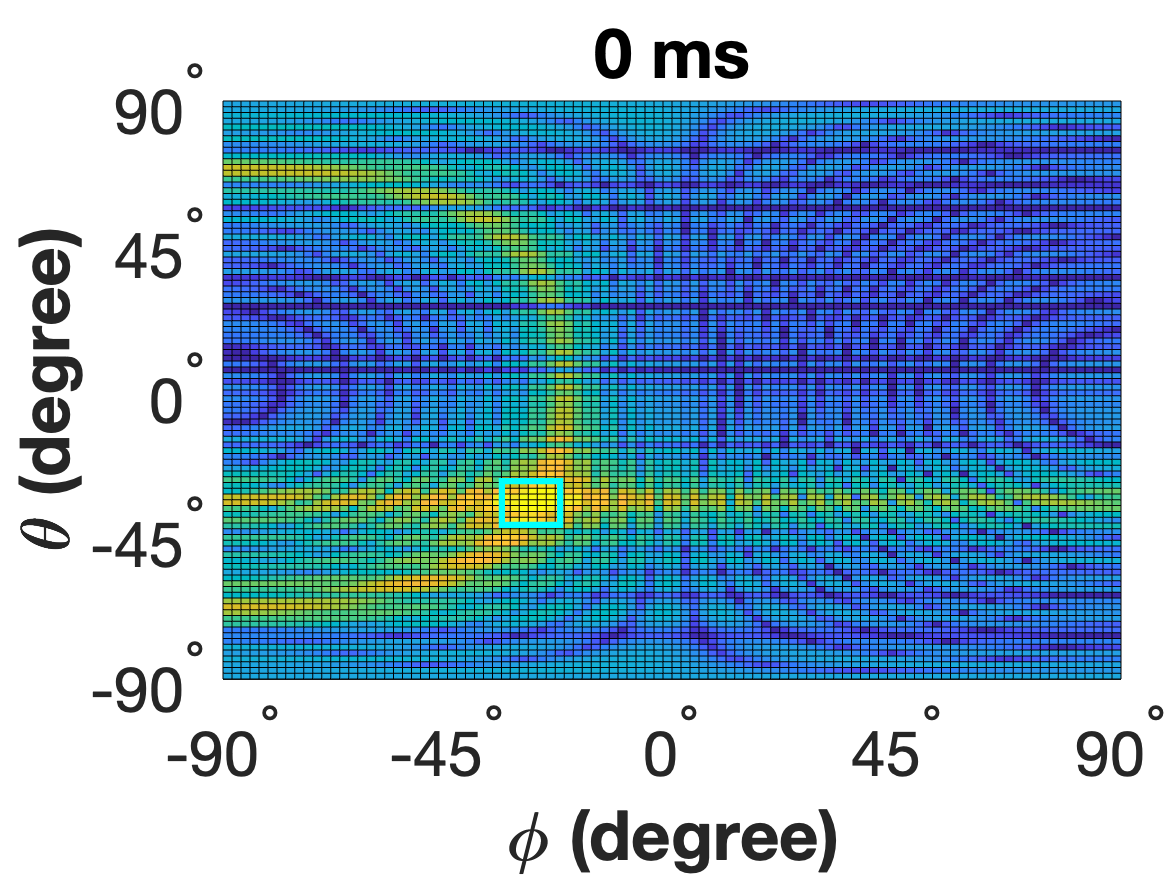
\includegraphics[width=\textwidth,height=3.5cm]{Figures/1LC_transition_3D.pdf}
   \end{minipage}
   \begin{minipage}[t]{0.19\textwidth}
     \centering
         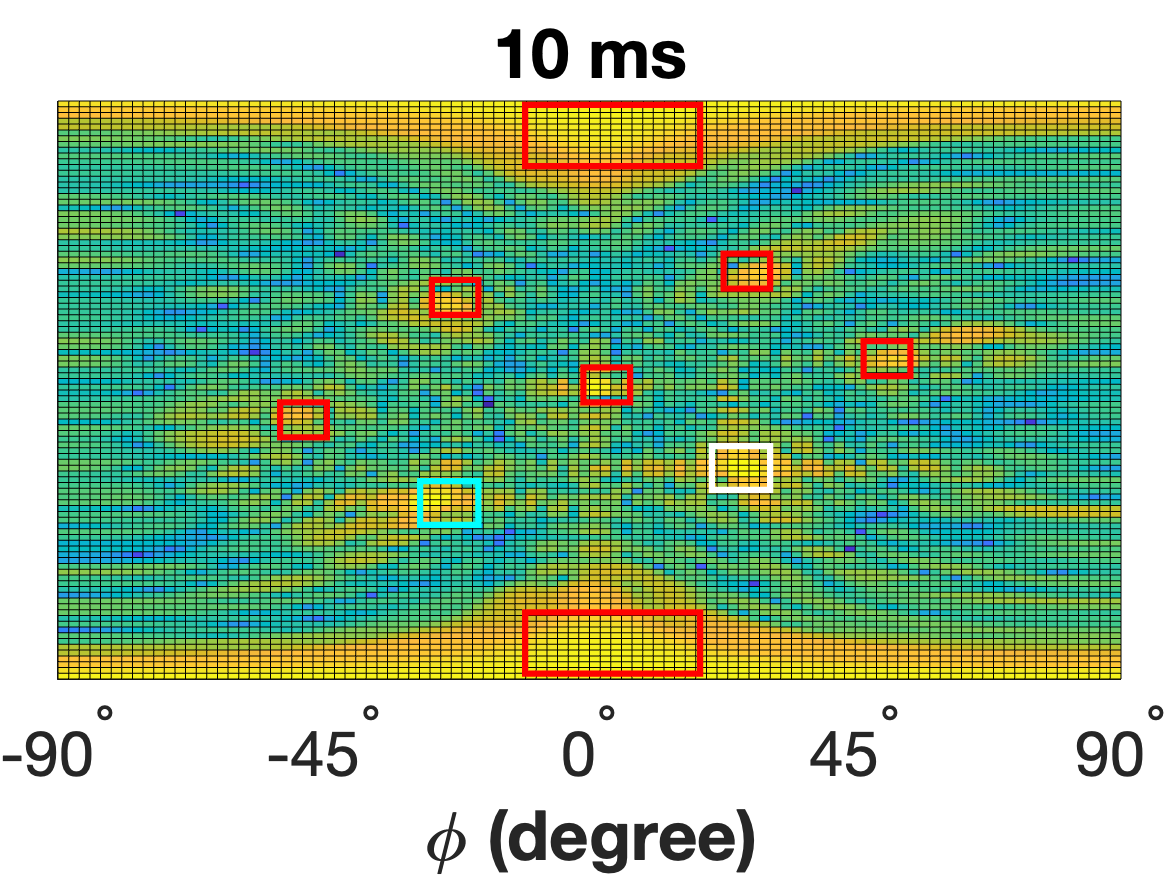
\includegraphics[width=\textwidth,height=3.5cm]{Figures/2LC_transition_3D.pdf}
   \end{minipage}
   \begin{minipage}[t]{0.19\textwidth}
     \centering
         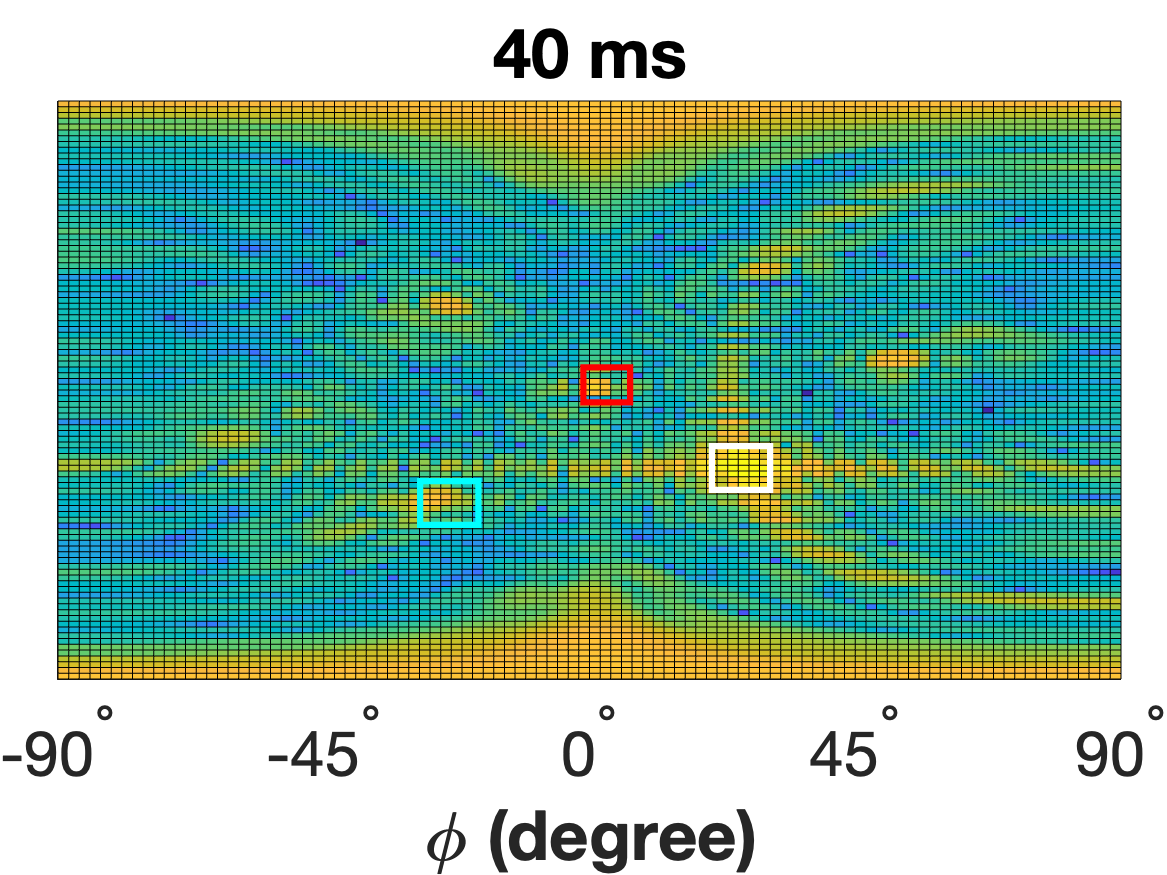
\includegraphics[width=\textwidth,height=3.5cm]{Figures/3LC_transition_3D.pdf}
   \end{minipage}
   \begin{minipage}[t]{0.19\textwidth}
     \centering
         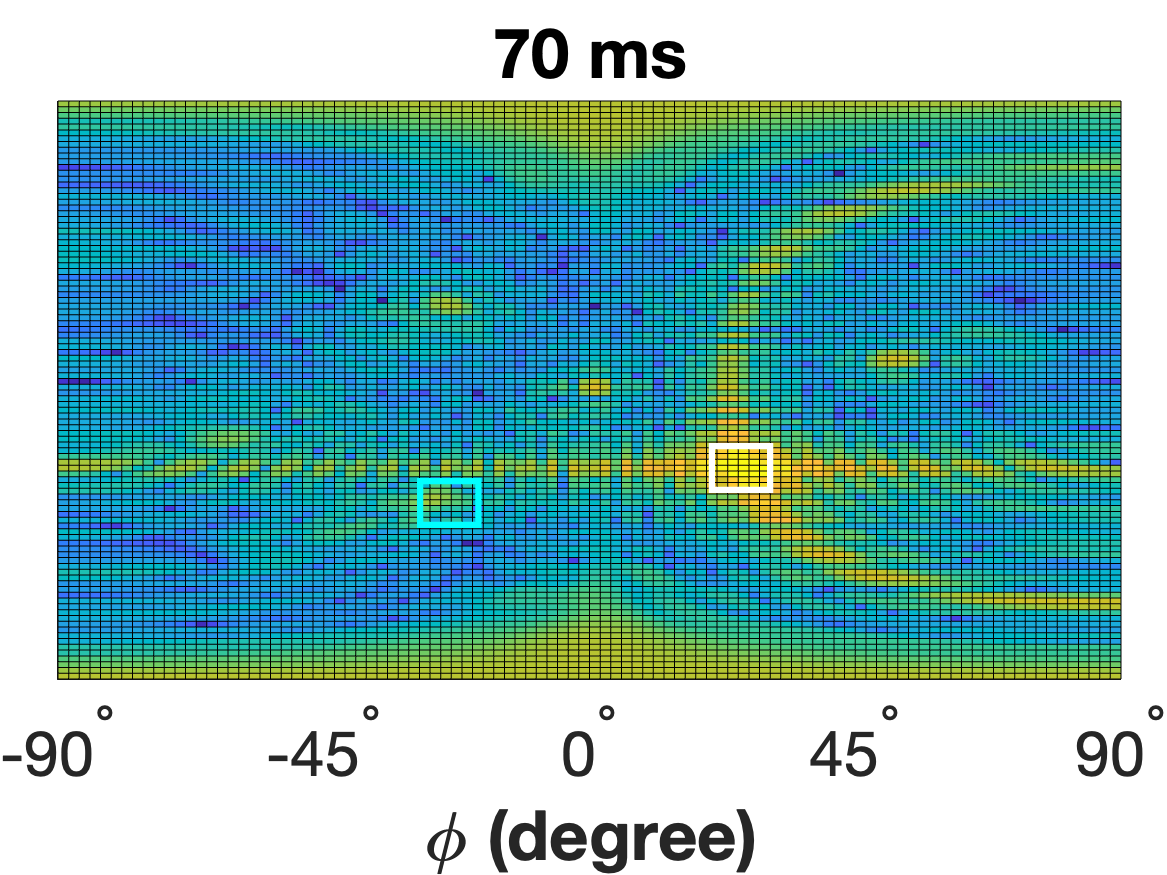
\includegraphics[width=\textwidth,height=3.5cm]{Figures/4LC_transition_3D.pdf}
   \end{minipage}
   \begin{minipage}[t]{0.205\textwidth}
     \centering
         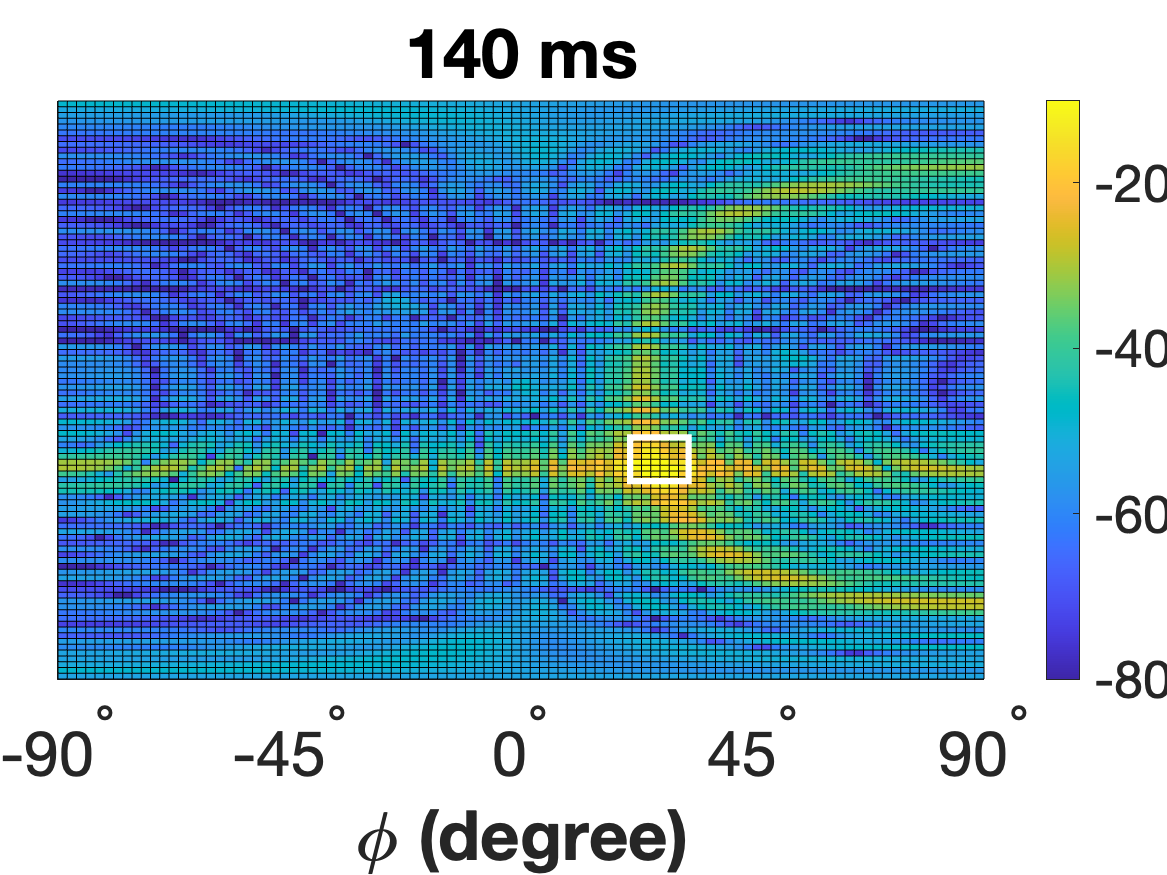
\includegraphics[width=\textwidth,height=3.5cm]{Figures/5LC_transition_3D.pdf}
   \end{minipage}
    \caption{\gls{NRCS} (in dB) at several time instances when transitioning from desired reflection angles $(\phi,\theta)=(-20,-30)$ to $(30,-20)$. Cyan, white, and red rectangles are showing the current, desired, and interference directions, respectively. The \gls{RIS} response time constants are for the \gls{PA} design in \cite{neuder2023compact} and the phase-shifts are based on the quadratic phase-shift design in \cite{jamali2021power}.}
    \label{fig:time response}
\end{figure*}

\subsection{Temperature-adaptive RIS configuration}\label{sec:temperature}
In an outdoor scenario, a \gls{RIS} needs to withstand a large range of temperatures.
For outdoor cellular systems, operation within \SIrange{-30}{+50}{\celsius} should be guaranteed. %\alejandro{does somebody know the right temperatures? It was -10 to 40, but that seems to narrow to me.}
As is illustrated in Fig.~\ref{fig:LCmolres}, the phase-shift vs. control voltage curve of the \gls{NLC}-\gls{RIS} is a function of temperature. This implies that a \gls{RIS} phase-shift configuration that is designed for temperatures in summer may not be applicable in winter. Hence, there is a need to develop temperature-aware phase-shift strategies. This requires the \gls{RIS} phase-shift behavior to be characterized offline and  the temperature to be estimated (e.g., by a thermometer deployed on the \gls{RIS}) during online operation for adapting the phase-shift design policy. Depending on the estimation error and update frequency of temperature information, robust designs that are valid for a range of temperatures may be required.


%\sout{In most cases, it can be distinguished between i) operation during the extreme temperatures, and ii) irreversible degradation of the performance after low or high temperatures have been reached. i) greatly depends on the \gls{NLC} chemical composition and can be tailored to certain applications. For example, the currently most commonly used GT7-29001 mixture has been characterized in the \SIrange{-10}{+80}{\celsius} temperature range \cite{tesmer2021temperature}. Below the minimum temperature, the material solidifies, but can be used after higher temperatures are reached again. For temperatures above \SI{999}{\celsius}, the \gls{NLC} becomes a conventional liquid and cannot be effectively tuned anymore. Furthermore, at high temperatures, a ii) progressive degradation of the organic components present in the \gls{NLC} occurs, so that the long-term performance is compromised even after cooler temperatures are reestablished.} \vahid{Such extreme temperatures is unlikely to happen in most cases. If we have space issues, we can consider removing this paragraph.}

\subsection{LC-RIS Design Tradeoffs}

In general, the maximum attainable phase-shift  of \gls{NLC} decreases with increasing temperature or decreasing frequency (see Fig.~\ref{fig:LCmolres}) \cite{tesmer2021temperature}. Therefore, to guarantee the full $360$-degree phase shift tuneability, one should design the \gls{RIS} unit cells for the maximum temperature and minimum operating frequency. This can be achieved in the \gls{PA} implementation by choosing a sufficiently large phase-shifter length $l_{\rm PS}$ (within the feasible range given the implementation constraints), since  the maximum phase-shift scales with $l_{\rm PS}$. However, as discussed in Section~\ref{Sec:Basic}, the insertion loss also scales with $l_{\rm PS}$.
Therefore, investigating the tradeoff among the maximum achievable phase shift, the resulting insertion loss, and the achievable performance (across the operating temperature and frequency) constitutes an interesting direction for future research.
To the authors' knowledge, this effect is not being considered and reported in current \gls{NLC}-\gls{RIS} designs.

%Moreover, the higher the temperature, the higher the insertion loss, and the lower the maximum attainable phase-shift  of \gls{NLC} (see Fig.~\ref{fig:LCresponse}) \cite{tesmer2021temperature}. , but this implies a larger insertion loss.
%Although the effect is very linear and not severe, it should be considered during the design of the \gls{RIS}'s phase shifters, so that 


\subsection{Biasing}
\label{ss:biasing}
For the realization of large \glspl{RIS}, the use of glass as a substrate is of great advantage due to the compatibility with current \gls{LCD} technology.
As in commercial \gls{LCD} displays, using \glspl{TFT} at each \gls{RIS} element to address them with $N+M$ (number of rows + columns) connecting lines instead of $N \times M$ (one line per element) is a meaningful approach to the challenge of biasing thousands or even millions of elements.
The additional challenge compared to common \glspl{LCD} is the higher capacitance of \gls{mm-Wave} circuits due to their larger size, requiring larger \glspl{TFT}. 
However, constraints might arise to minimize the effect of the bias lines in the \gls{RIS} operation.
This poses an additional challenge in the design of element-wise tunable \glspl{RIS} using the \gls{RA} method, since the bias lines will affect the performance of the radiating elements. 
This is commonly solved by biasing lines perpendicular to the electric-field polarization which is only possible for single, linearly polarized operation. Dual polarization designs require alternative solutions that account for the effect of the biasing lines when designing the radiating elements.
In the \gls{PA} method, this is not an issue due to the separation of the phase shifters and the radiating elements in different layers.


%\textcolor{red}{Using Indium Tin-Oxide (ITO) for the electrode feeding lines is the standard present in nearly every display due to its transparency to light.
%Nevertheless, an \glspl{RIS} does not need to be transparent to light (around 400-800 THz) but to much lower frequencies, so that novel, cheaper materials may be investigated which satisfy the requirements for low resistivity and can be cost-effectively grown (e.g., sputtered) on large surfaces.}
%\textcolor{blue}{A solution could be achieved using vias (i.e., interconnects between different layers) to bring the electrode biasing lines to an additional, RF-decoupled layer.
%Realizing through glass vias for RF circuits has been a topic of research for more than a decade, and important advances have been achieved \cite{watanabe2020ultrathin}. 
%Despite possible, the technique is not yet cost-effective for the realization of large panels.
%For this reason, the incorporation of the electrode feeding lines for the LC tuning should be achieved within the same layer as the electrodes themselves, potentially interfering with the incident, guided, and reflected electromagnetic fields.}
%\alejandro{Both colored parts could be removed to keep it short. I guess I went too much into detail.}
%\vahid{I agree that we have to make the discussion more concise. However, can we "add" a sentence about whether the biasing approach has an impact on RIS optimization? perhaps in terms of control capability?}

\subsection{Bandwidth}

\glspl{RIS} can be designed to support a single service provider (i.e., limited part of the band); an entire frequency band (e.g., 5G \SIrange{26.5}{29.5}{\giga\hertz} band), or even several bands, for example, the \SI{28}{\giga\hertz} and \SI{60}{\giga\hertz}. 
For high bandwidth systems, operating in a single band, the \gls{PA} implementation is more suitable compared to the \gls{RA}. However, \gls{RA} implementation is more suitable for multi-band operations due to the simplicity of their design. However, this comes at the cost of higher response time. Moreover, the phase-shift vs. voltage control curve of \gls{NLC}-\glspl{RIS} (see Fig.~\ref{fig:LCmolres}) changes across different frequencies within the band. Therefore, wideband phase-shift designs that exploit the frequency-dependent characteristics of the \gls{NLC}-\glspl{RIS} have to be developed.%needed in a single band, the higher the suitability of the phased array method compared to the reflectarray method. 
%In case of iii) multi-band applications, integrating multiple phase shifters in the phased array method will become an extra design effort, so the reflectarray method would be a simpler solution as long as the slower response times can be tolerable for the targeted application. Nevertheless, for wideband operations (especially scenario iii), the phase-shift vs. voltage control curve of LC-RISs (see Fig.~\ref{fig:LCresponse}) changes across different frequencies within the band. Therefore, wideband phase-shift designs that exploit the frequency-dependent characteristics of the LC-RISs have to be developed.
% \section{Outlook: Applications in Wireless Communications}
\label{sc:applications}
The applications of \glspl{RIS} in wireless networks have been extensively discussed in the literature~\cite{liu2021reconfigurable}. The existing work on \glspl{RIS} can be divided into three categories, namely, \gls{RIS} for communication, \gls{RIS} for localization and sensing, and \gls{RIS} for privacy and security. In the following, we elaborate on the potential of \gls{NLC} in each category. 

\textbf{RIS for communication.} The majority of literature focuses on leveraging \glspl{RIS} to enhance various aspects of communications systems, including capacity~\cite{bRISSR}, energy efficiency~\cite{bRISEE}, and fairness~\cite{bRISUF}. The use-cases for these studies vary from the traditional cellular network to vehicular~\cite{liu2020machine}, aerial~\cite{chen2022reconfigurable}, and industrial~\cite{dhok2021non} use-cases. 

The advantages of continuous phase-shift tunability in \gls{NLC} are two-fold: $(i)$ they do not have the typical performance losses from discrete phase shift selection, which is particularly important in MIMO systems, and $(ii)$ optimizing the \gls{RIS} configuration is less complex with \glspl{NLC}, since phases are optimized as continuous variables, as opposed to discrete variables. 

Given the limitation in response time, \gls{NLC} is not suitable for applications with high mobility. For example, a user at a \SI{50}{\meter} distance from a \gls{RIS} projecting a beamwidth of 5$^\circ$ can move \SI{2.18}{\meter} (perpendicular to the boresight) without stepping out of the beam's coverage. Assuming that the user moves at \SI{72}{\kilo\meter/\hour}, with \gls{NLC} phase shifters with a tuning time of \SI{10}{\milli\second}, we need to repeat the beam refinement procedure at every 10 frames in 5G systems. This limitation can be addressed through algorithmic as well as system design choices, such as using multiple \glspl{RIS} or leveraging proactive and progressive beamsteering based on user's trajectory. 

\textbf{RIS for localization and sensing.} This is another interesting application area of \glspl{RIS} which is relatively under-explored. For localization, \glspl{RIS} are used as virtual anchors whose location is known~\cite{emenonye2022fundamentals}. Similarly, \glspl{RIS} can enhance sensing by controlling the multi-path signals for better illumination of the target~\cite{hu2020reconfigurable}. In both cases, the discrete nature of \gls{RIS} phase configuration is considered a limitation \cite{keykhosravi2021multi}, which \glspl{NLC} can alleviate. For accurate location and sensing, the \gls{RIS} should have a \gls{LOS} link to the target, which essentially requires a dense deployment. The cost-effective nature of \glspl{NLC} plays an important role in this regard. 

\textbf{RIS for security.} The steering and phase manipulation capability of \glspl{RIS} is particularly interesting for physical layer security, where the \gls{RIS} can direct interference in the form of out-of-phase reflections of the signal towards the eavesdropper, hence, increasing the secrecy rate of the communication. Here, discrete phase shifts not only reduce the effectiveness of the scheme against eavesdropping, but also an eavesdropper with the knowledge of the discrete states might be able to reverse the impact of \gls{RIS}. Hence, \glspl{NLC} are again more effective in enhancing physical layer security. 

% \begin{itemize}
%     \item RIS for communication. The  (blockages, reducing BS density)
%     \item RIS for localization and sensing (higher density, less issue with occlusions, esp at higher frequencies)
%     \item RIS for privacy and security (Controlling the environment, avoiding jammers from directions that signal is not intended to come or privacy?) or physical layer security by sending noise towards non-receiver direction.

% \end{itemize}
\section{Conclusion}
\label{sc:conclusion}

This paper presented \gls{NLC} as an enabler technology for building extremely large \glspl{RIS} with continuous tuning capability, low power consumption, frequency scalability, and cost-efficient fabrication. However, these advantages come with the limitations such as slow response time and temperature dependencies. The basic physical principles of \gls{NLC} theory were reviewed and two important implementations of \gls{NLC}-\glspl{RIS} were introduced. Finally, \gls{NLC}-\glspl{RIS} were compared against competing technologies \gls{SC}- and \gls{MEMS}-\glspl{RIS} and several important open research problems on  \gls{NLC}-\glspl{RIS} were presented. 





\ifCLASSOPTIONcaptionsoff
  \newpage
\fi

\bibliographystyle{IEEEtran}

\bibliography{literature}

\section{Acknowledgements}
This research was partly funded by the Deutsche Forschungsgemeinschaft (DFG, German Research Foundation) – Project-ID 287022738 – TRR 196 MARIE within project C09, by the mm-Cell project and the Collaborative Research Center 1053 MAKI, and by the LOEWE initiative (Hesse, Germany) within the emergenCITY center.

\section*{Biography}
\noindent 
\textbf{Alejandro Jim\'enez-S\'aez} is a Research Group Leader at the Institute of Microwave Engineering and Photonics (IMP) at the Technical University of Darmstadt (TUDa), Darmstadt, Germany. His research interests include RF components based on artificial and functional materials.

\vspace{0.3cm}
\noindent 
\textbf{Arash Asadi} (Senior Member, IEEE) is a Research Group Leader at TUDa, where he leads the Wireless Communication and Sensing Lab (WISE). His research interests include wireless communication and sensing and its application in beyond-5G/6G networks. %He was a recipient of several awards, including the Athena Young Investigator Award from TU Darmstadt and the Outstanding Ph.D. and Master’s Thesis Awards from UC3M. Some of his papers on D2D communication have appeared in IEEE Communications Society’s (COMSOC) best reading topics on D2D communication and IEEE Communications Society's (COMSOC) Tech Focus. He continuously contributes to the community through participation in TPCs and organizing committees such as IEEE INFOCOM, ACM MobiCom, and IEEE ICNP.

\vspace{0.3cm}
\noindent 
\textbf{Robin Neuder} is a Ph.D. student at IMP, TUDa, Darmstadt, Germany.

\vspace{0.3cm}
\noindent 
\textbf{Mohamadreza Delbari} is a Ph.D. student at the Resilient Communication Systems (RCS) Lab at TUDa, Darmstadt, Germany.

\vspace{0.3cm}
\noindent 
\textbf{Vahid Jamali} is an Assistant Professor leading the RCS Lab at TUDa, Darmstadt, Germany. His research interests include wireless and molecular communications.


% \vspace{0.3cm}

% To do/check:
% \begin{itemize}
% \item Let's check if a biography is still mandatory. If not, we can drop it.

% \item Intro: \ara{@AJS:Is there something with mems?}

% \item RA: \ara{we should unify response time and tuning time. AFAIK they are the same right?}

% \item Notation: consistent use of phase-shifter (or phase shifter), response time (or tuning time)

% \item SC: \ara{@AJS: Don't we mention temp as a challenge for LC-RIS?}

% \item MEMS: \ara{@AJS: is this discrete?}

% \item Overhead: \ara{@VJ: One can argue the overhead remains the same. In the end, the mmWave 5G NR has all these procedures in the standard. } 

% \item Fig. 4: \ara{I would suggest 1) arranging the figures page wide, reducing the size of the figures by ~30-50\%, increasing the number of figures according to see the transitions and then adding some labels on the figure showing the current and desired direction and perhaps a red circle around the interference directions.} \vahid{@MD: I agree with Arash, you can consider 5 figures in a row to better illustrate the transition.}

% \item Fig. 4: \vahid{@MD: In addition to the comments by Arash, please ensure that the figure data is consistent with the text. There, it is stated that NRCS (in dB) is plotted, is this what we plot in Fig. 4? The numbers seem too low to me. Please add the values for the desired reflection angles in the caption.}

% \end{itemize}



% \textbf{Word track:} Here is a potential organization outline, we can keep improving it:

% \begin{itemize}
% \item \textbf{Abstract:} \textcolor{red}{($\approx 100-150$ words)}
% \item \textbf{Section~I:} Introduction \textcolor{red}{($\approx 500-800$ words)}
% \begin{itemize}
% \item Promises of RISs and the need for hardware implementation
% \item A brief statement of existing technologies and motivation for cost-effective LC technology for large RISs
% \item The focus of this magazine, namely the underlying physics of LC, key features and limitations, comparison with other technologies, and future research directions
% \end{itemize}
% \item \textbf{Section~II:} LC-based RIS technology \textcolor{red}{($\approx 1200-1800$ words)}
% \begin{itemize}
% \item Physical operating principles
% \item Reflect-array-based implementation
% \item Phased-array-based implementation
% \end{itemize}
% \item \textbf{Section~III:} Comparison with other RIS technologies \textcolor{red}{($\approx 1200-1800$ words)}
% \begin{itemize}
% \item PIN-diodes: brief description, advantages, and limitations
% \item RF switches: brief description, advantages, and limitations
% \item MEMS: brief description, advantages, and limitations
% \item LC: advantages, limitations, and summary
% \end{itemize}
% \item \textbf{Section~IV:} Future research directions \textcolor{red}{($\approx 800-1000$ words)}
% \begin{itemize}
% \item Beam-design for slow LC-based RISs
% \item Phase-shift range vs. insertion loss (or in Section II)
% \item Temperature-aware phase-shift designs
% \item Low-cost but imperfect hardware?
% \item Other hardware-related research items? impedance matching, biasing, etc.
% \end{itemize}
% \item \textbf{Section~V:} Conclusions \textcolor{red}{($\approx 100-150$ words)}
%     \item \textbf{References:} \textcolor{red}{($\approx 300-400$ words)} We have to choose $15$ references that are representative of the literature (including our contributions) and well fit the flow of the paper. 
%     \item \textbf{Biography:} \textcolor{red}{($\approx 500-700$ words)}
% \end{itemize}

% \textbf{Total word count:} \textcolor{red}{($\approx 4700-6800$ words)} where we have to stick to \textcolor{red}{$\approx 5500$ words)} 

% \textbf{Figures:} We may include only 6 figures/tables. My suggestions are:
% \begin{itemize}
% \item Table comparison
% \item Figure for alternative technologies, we probably need, too
% \item We need one figure for simulation results
% \item We need at least one figure to show the LC principle. I suppose Figs. 2 and 3 can be combined. Fig. 4, we have to keep if both implementations are discussed, otherwise, we can drop it.
% \item We may keep the overview figure (Fig. 1)
% \end{itemize}

% \begin{figure}[htp]
% 	\centering
%     \subfloat[]{
% 		\includegraphics[width=\columnwidth]{Figures/Method_Reflectarray.pdf}
% 		\label{fig:method_Reflectarray}
%     } 
%     \hfill
%     \subfloat[]{
% 		\includegraphics[width=\columnwidth]{Figures/Method_PhasedArray.pdf}
% 		\label{fig:method_PhasedArray}
%     }
%     \caption{Two prospective methods for the realization of \glspl{RIS}. a) Reflectarray method. b) Phased array method. \vahid{Is the main difference on each unit-cell level or also on their connection? We say that for (a) we do not need the pattering of the ground layer.}
%     \alejandro{Other than the layer in which it is done, the connection for biasing is similar in both cases}}
%     \label{fig:methods_RIS} 
% \end{figure}

% \begin{figure}[t]
% 	\centering
% 	\subfloat[]{
%         \includegraphics[height=0.195\columnwidth]{Figures/IMSL_biased.pdf}
%         \label{fig:IMSL_biased}
%     }
% 	\subfloat[]{
% 		\includegraphics[height=0.195\columnwidth]{Figures/IMSL_unbiased.pdf}
% 		\label{fig:IMSL_unbiased}
%     }
%     \caption{\ara{it would be nice to have a figure that show the "path" better and how the orientation of molecules impact the phase shift} \vahid{Agreed, to essentially show the path where the wave is impinged, phase-shifted, and reflected.} Biasing mechanism for the controlled rotation of \gls{NLC} molecules. a) By applying a \gls{DC} or low frequency (usually \SI{1}{\kilo\hertz}) voltage to the top and bottom electrodes, the molecules are aligned in parallel with the E-field lines of the \gls{RF}-field, $\varepsilon_{r, \parallel}$. b) When the biasing is removed, anchoring forces due to a surface patterning of thin alignment layers align the \gls{NLC} molecules in the perpendicular state, $\varepsilon_{r, \perp}$.}
%     \label{fig:LC_planar_2electrodes}
% \end{figure}

\end{document}


